\documentclass[]{article}

%Change helvetica
\usepackage[scaled]{helvet}
\renewcommand*\familydefault{\sfdefault} %% Only if the base font of the document is to be sans serif
\usepackage[T1]{fontenc}

%Set page width 
\usepackage[textwidth=16cm]{geometry}

%Used to improve the headers
\usepackage{fancyhdr}

%Used to include images into the document
\usepackage{graphicx}

%Used to make some pages landscape
\usepackage{lscape}

%Used to wrap figures in text
\usepackage{wrapfig}

%Translate LaTeX terms to dutch
\usepackage[dutch]{babel}

%Used to display url's
\usepackage{hyperref}

%Used to calculate last page
\usepackage{longtable}

%Used to display "normal" paragraph's without indentation and with blank line
\usepackage[parfill]{parskip}

%Don't break paragraphs in page
\widowpenalties 1 10000
\raggedbottom

%Stop wordbreaking
%\usepackage[none]{hyphenat}

%Use \insertdate to insert current formatted date
\makeatletter
\let\insertdate\@date
\makeatother

%Stop word breaks
\tolerance=1
\emergencystretch=\maxdimen
\hyphenpenalty=10000
\hbadness=10000

%add version command, use \version to insert current version
\newcommand{\version}{1.15}

% Alter some LaTeX defaults for better treatment of figures:
% See p.105 of "TeX Unbound" for suggested values.
% See pp. 199-200 of Lamport's "LaTeX" book for details.
%   General parameters, for ALL pages:
\renewcommand{\topfraction}{0.9}    % max fraction of floats at top
\renewcommand{\bottomfraction}{0.8} % max fraction of floats at bottom
%   Parameters for TEXT pages (not float pages):
\setcounter{topnumber}{2}
\setcounter{bottomnumber}{2}
\setcounter{totalnumber}{4}     % 2 may work better
\setcounter{dbltopnumber}{2}    % for 2-column pages
\renewcommand{\dbltopfraction}{0.9} % fit big float above 2-col. text
\renewcommand{\textfraction}{0.07}  % allow minimal text w. figs
%   Parameters for FLOAT pages (not text pages):
\renewcommand{\floatpagefraction}{0.7}  % require fuller float pages
% N.B.: floatpagefraction MUST be less than topfraction !!
\renewcommand{\dblfloatpagefraction}{0.7}   % require fuller float pages

\pagestyle{fancy}

\fancyhead{}
\fancyfoot{}

\fancyhead[L]{Melroy van den Berg \& Vincent Kriek}
\fancyhead[R]{
\includegraphics[height=30pt,keepaspectratio]{tassbw.pdf}}

\fancyfoot[L]{DomoTop - Afstudeerverslag}
\fancyfoot[C]{\thepage\space van \pageref{lastpage}}
\fancyfoot[R]{v\version}

% Add line above footer
\renewcommand{\footrulewidth}{0.4pt}% default is 0pt

\begin{document}


\title{\textbf{DomoTop} \\Afstudeerverslag}
\author{Vincent Kriek \and Melroy van den Berg}

\maketitle

\thispagestyle{empty}
\begin{figure}[htpb]
   \begin{center}
    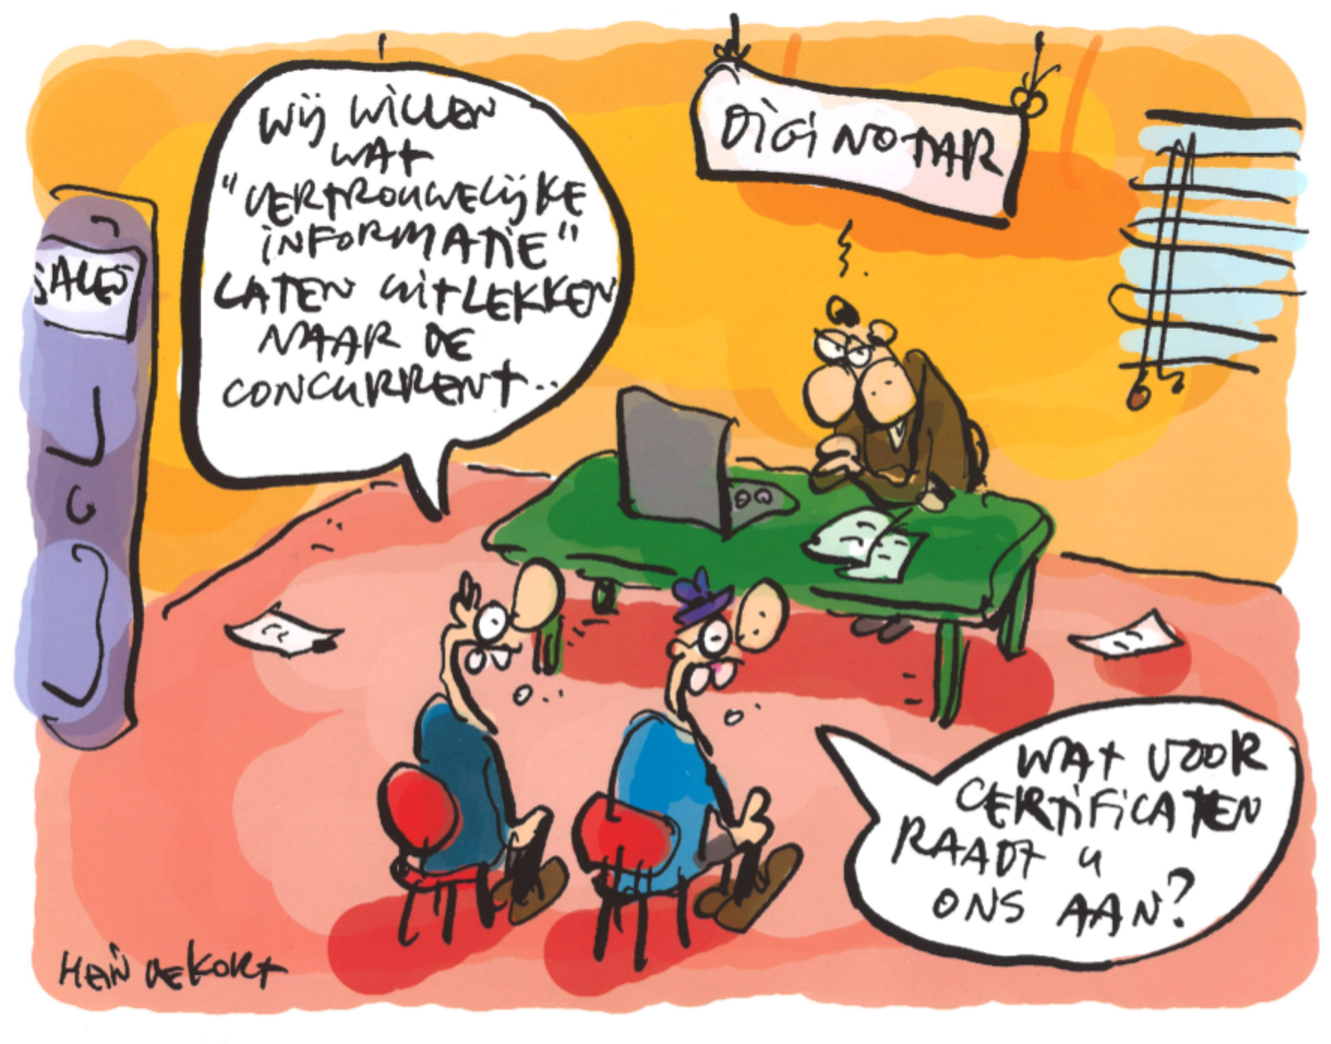
\includegraphics[width=0.8\textwidth]{voorkant.pdf}
   \end{center}
\end{figure}

%\vspace*{-3cm}
\vspace*{\fill}

\newpage
\thispagestyle{empty}

\noindent\copyright  TASS B.V. 2011
Alle rechten voorbehouden. Verveelvuldiging, geheel of gedeeltelijk, is
niet toegestaan dan met schriftelijke toestemming van de
auteursrechthebbende.
All rights are reserved. Reproduction in whole or in part is prohibited
without the written consent of the copyright owner. Dit document is
gepubliceerd door:\\
TASS BV\\
Eindhoven, Nederland\\

\noindent Commentaar en suggesties kunnen worden gestuurd naar:\\
\indent TASS B.V.\\
\indent\indent Postbus 80060\\
\indent\indent 5600 KA  EINDHOVEN\\
\indent\indent Nederland\\
\indent\indent tel:  +31 40 2503200\\
\indent\indent fax:  +31 40 2503201\\

\vspace*{\fill}

\begin{tabular}{|| l | l || l | l ||}\hline
   Document ID: & AFVSL-MV-21          &Project naam:     &DomoTop             \\\hline
   Datum:       &14 mei 2012          &School begeleider:&Peter Kailuhu       \\\hline
   Versie:      &\version              &People Manager:   &Gerben Blom         \\\hline
   Status:      &concept               &Documentnaam:     &Afstudeerverslag.pdf\\\hline
   Auteur:      &Melroy van den Berg \&&Reviewer:         &Gerben Blom         \\
                &Vincent Kriek         &                  &                    \\\hline
   Printdatum:  &\insertdate           &Classificatie:    &Openbaar            \\\hline
\end{tabular}

\newpage
\thispagestyle{empty}
\section*{Geschiedenis}

\begin{tabular}{|| l | l | l | l ||}\hline
    Versie  &Datum       &Auteur              &Beschrijving                    \\\hline\hline
    0.1     &02-03-2012  &Vincent Kriek \&    &Init opzet                      \\
            &            &Melroy van den Berg &                                \\\hline
    0.2     &02-03-2012  &Vincent Kriek       &Hoofdstuk 2, eerste versie      \\\hline
    0.3     &05-03-2012  &Melroy van den Berg &Plan van Aanpak, Verklarende    \\
            &            &                    &woordenlijst + review           \\
            &            &                    &probleemanalyse                 \\\hline
    0.4     &05-03-2012  &Vincent Kriek       &Probleemanalyse, methoden en    \\
            &            &                    &technieken                      \\\hline
    0.5     &04-04-2012  &Melroy van den Berg &Methoden en technieken verder   \\
            &            &                    &gespecificeerd en uitvoering    \\
            &            &                    &verder uitgebreid               \\\hline
    1.01    &04-04-2012  &Melroy van den Berg &Concept verslag aangekondigd    \\\hline
    1.02    &04-04-2012  &Vincent Kriek       &Resultaten eerste versie        \\\hline
    1.03    &04-04-2012  &Vincent Kriek       &Feedback Peter verwerkt         \\\hline
    1.04    &08-04-2012  &Vincent Kriek       &Eerste versie document in \LaTeX\\\hline
    1.05    &09-04-2012  &Vincent Kriek       &Verslag compleet in \LaTeX      \\\hline
    1.06    &10-04-2012  &Melroy van den Berg &Uitvoering geschreven           \\\hline
    1.07    &25-04-2012  &Melroy van den Berg &Uitvoering uitgebreid           \\\hline
    1.08    &26-04-2012  &Vincent Kriek       &Resultaten uitgebreid           \\\hline
    1.09    &04-05-2012  &Melroy van den Berg &Uitvoering + Methoden \&        \\ 
            &            &                    &Technieken uitgebreid           \\\hline
    1.10    &14-05-2012  &Melroy van den Berg &Conclusie + Inleiding +         \\
            &            &                    &Samenvatting geschreven         \\\hline 
    1.11    &14-05-2012  &Vincent Kriek       &Voorwoord                       \\\hline
    1.12    &21-05-2012  &Vincent Kriek       &Voorwoord verbeterd             \\\hline
    1.13    &24-05-2012  &Melroy van den Berg &Document lay-out verbeterd      \\\hline
    1.14    &04-06-2012  &Melroy van den Berg &Reviews doorvoeren	           \\\hline
    1.15    &04-06-2012  &Vincent Kriek       &Uitvoering uitgebreid           \\\hline
\end{tabular}

\newpage
\thispagestyle{empty}
\section*{Voorwoord}
\addcontentsline{toc}{section}{Voorwoord}
Domotica systemen nemen een steeds prominentere plaats in in de huidige
samenleving. Denk bijvoorbeeld aan de Living Colors lampen van
Philips\textsuperscript{\texttrademark}, het
KlikAanKlikUit\textsuperscript{\textregistered} systeem dat je voor twee
tientjes bij de Blokker haalt en de nieuwe
Toon\textsuperscript{\textregistered} van Eneco. Maar wat voor soort beveiliging
zit er op zulke systemen?  En wat voor beveiling zou het meest geschikt zijn? In
onze stage hebben we bekeken wat de beste beveiliging is voor dit soort
systemen.

In de presentatie kan niet alles getoond worden dat er is gedaan en bereikt
tijdens de afstudeerstage. Om alles toch goed toe te lichten hebben we dit
verslag opgesteld.  Onze docenten, gecommiteerde en andere ge\"intresseerden
kunnen in dit verslag nalezen hoe wij onze stage hebben aangepakt, welke
methodes en technieken gebruikt zijn en wat voor resultaten we hebben
bereikt.

Voor de stage was onze kennis van beveiliging nog beperkt,
maar tijdens onze stage hebben we veel geleerd over dit vakgebied. Samen met
Berry Borgers, \'e\'en van onze technische begeleiders, hebben we een aantal keuzes
gemaakt over hoe we het project aan zouden pakken. Het onderzoek dat hieraan
vooraf ging heeft, samen met de stage, ons veel geleerd over beveiliging.

Het beveiligen van OpenRemote was voor TASS tweeledig. Ons project is bedoeld als
demonstratieproject op beurzen en scholen. Hiermee is aan te tonen wat er
allemaal mogelijk is op domotica gebied en welke rol beveiliging daarin speelt.
Tevens was het een onderzoeksproject, om te kijken hoe een domoticasysteem
het best beveiligd kan worden zonder in te leveren op het gebied van
gebruiksvriendelijkheid.

We willen Gerben Blom bedanken voor alle begeleiding die we op projectmatig vlak
gekregen hebben. Tevens willen we Berry Borger bedanken voor de technische
beleiding, informatie en advies op security gebied, alsmede Bas Burgers voor advies en begeleiding op technisch gebied. Ook willen we onze
begeiding vanuit school bedanken, met in het bijzonder Peter Kailuhu voor
de coachingsgesprekken en informatie over de eisen vanuit school.

\newpage
\thispagestyle{empty}
\tableofcontents
\thispagestyle{empty}
\newpage
\thispagestyle{empty}
\listoftables
\listoffigures

\newpage
\section*{Samenvatting}
\addcontentsline{toc}{section}{Samenvatting}
Het software project genaamd OpenRemote is uitgebreid met een beter
beveiligingssysteem dan voorheen. OpenRemote is een software
pakket om een domotica systeem op te zetten. Er wordt gebruik gemaakt van
een PlugTop computer om hierop de OpenRemote Controller te draaien, welke functioneert als
zijnde een server. Vandaar de projectnaam DomoTop (Domotica PlugTop).
De beveiligingstechniek die gebruikt wordt in het DomoTop project is SSL/TLS,
waarin gebruik wordt gemaakt van client certificaten om de
gebruikers/apparaten te authenticeren. Ook is er later in het DomoTop project
voor gekozen om de mogelijkheid te geven groepen aan te maken, waardoor
apparaten in een specifieke groep geplaatst kunnen worden. Hierdoor
is het dus mogelijk om apparaten te autoriseren.

Deze opdracht is afkomstig en bedacht door het bedrijf TASS. De opdracht wordt
begeleid door de people manager Gerben Blom, technische begeleiders Berry
Borgers en Bas Burgers. Deze stageopdracht is gevonden via Avans Den
Bosch bij een bedrijvenbeurs te Rotterdam. De opdracht is aangenomen door
Melroy van den Berg \& Vincent Kriek.

TASS vond het belangrijk om OpenRemote software te beveiligen en een oplossing
te vinden van een authenticatie mechanisme zonder gebruik te hoeven maken van
een gebruikersnaam/wachtwoord. OpenRemote is een software
applicatie, specifiek bedoeld om een domotica systeem op te zetten. OpenRemote
bestaat uit drie verschillende onderdelen: OpenRemote Modeler, OpenRemote
Controller en tot slot de OpenRemote Client. Met de OpenRemote Modeler kan er een ontwerp
gemaakt worden. Via de Controller worden commando's van de gebruiker
afgehandeld. Deze commando's zijn acties die gedaan moeten worden door de
OpenRemote Controller, bijvoorbeeld 'licht aan' van een bepaalde lamp. De OpenRemote Client, meestal een mobiel apparaat, stuurt
commando's naar de controller. Zie figuur \ref{global} voor een globaal overzicht van de
werking van OpenRemote.

Verder was het belangrijk dat er ervaring en onderzoek werd gedaan naar een PlugTop computer, waarop de OpenRemote Controller
draait. Tot slot was ook onderzoek nodig naar diverse domotica
protocollen en verschillende manieren van beveiligen. Hierdoor is kennis en
ervaring opgedaan op gebied van onder andere domotica, Google Android, Embedded
Linux, maar ook zijn er verschillende onderzoeksrapporten geschreven met
onderzoekresultaten. De meeste kennis is verkregen op gebied van SSL/TLS (Secure Sockets Layer),
waar onderzoek naar gedaan is. In dit onderzoek is gebleken dat SSL/TLS
de beste manier is om OpenRemote te beveiligen, daarnaast is er onderzocht hoe
SSL het beste ge\"implementeerd kon worden binnen het DomoTop project. 

Op dit moment is OpenRemote beveiligd via client certificaten en kan de
administrator via het OpenRemote administrator panel apparaten goed-/afkeuren.
Het administrator panel is een webbased applicatie en behoort tot de OpenRemote
Controller. Op de OpenRemote Modeler kunnen er groepen gemaakt worden en
gekoppeld worden aan knoppen, sliders en/of switches, waarna je deze groepen in
het administrator panel kan koppelen aan apparaten.

\begin{figure}[htpb]
   \begin{center}
     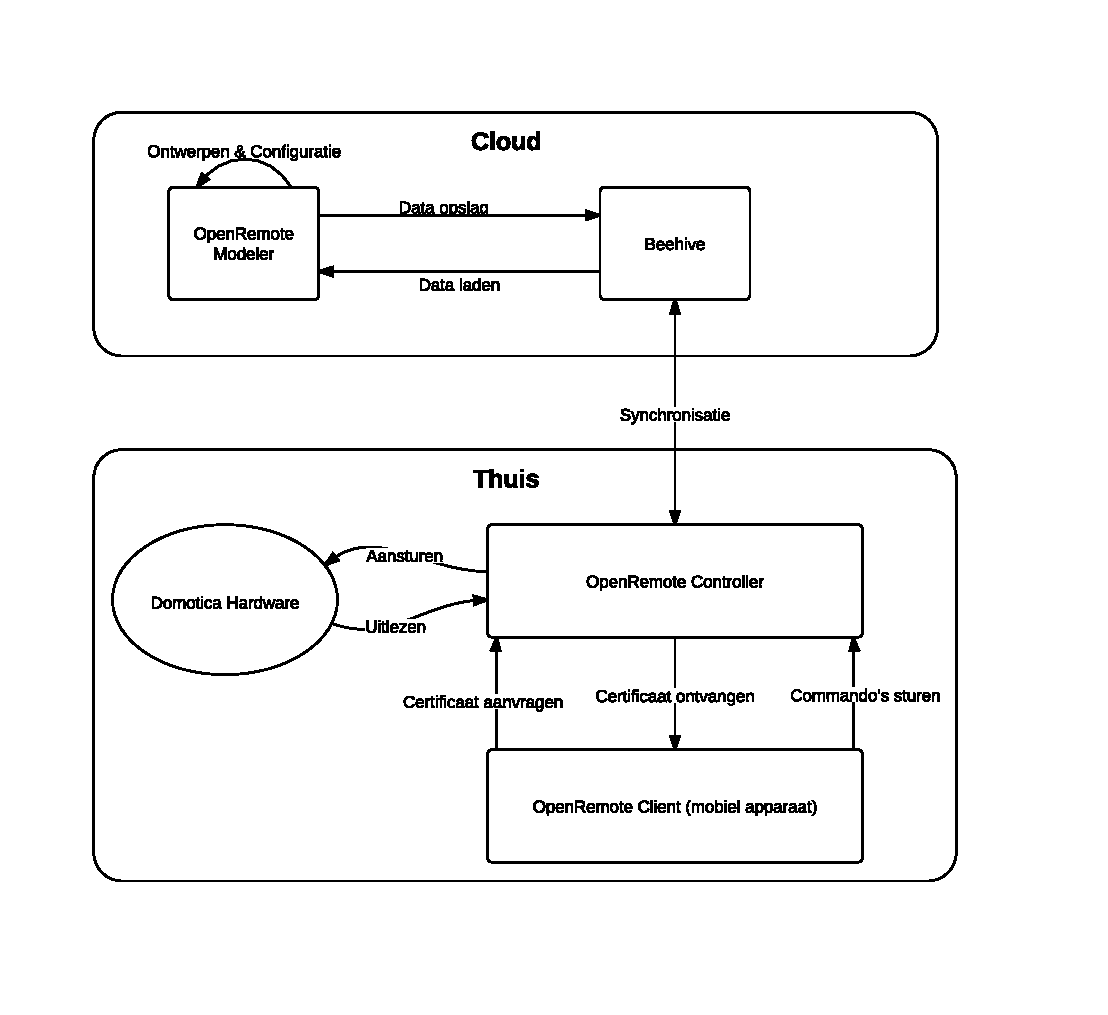
\includegraphics[width=\textwidth]{GlobalOR.pdf}
   \end{center}
   \caption{Globale werking van OpenRemote}
   \label{global}
\end{figure}

\newpage
\section{Inleiding}
Vandaag de dag merk je dat beveiliging een steeds belangrijkere rol krijgt binnen
de samenleving, er wordt immers veel gesproken over beveiligingskwesties in
het nieuws. Zo werd KPN gehackt, dit keer door een 17-jarige jongen, en
er werden weer allerlei persoonlijke gegevens en/of logingegevens verspreid via het
internet.

In dit verslag wordt besproken hoe het met de beveiliging is gesteld bij een
softwareapplicatie genaamd OpenRemote. OpenRemote is een applicatie die
bedoeld om thuis een (eigen) domotica systeem op te zetten. Deze applicatie
bestaat uit verschillende onderdelen. De OpenRemote Controller is het hart van
het pakket. Deze draait op een server binnenshuis en op deze server wordt de
domotica apparatuur aangesloten. Om de domotica apparatuur aan te spreken wordt
er gebruik gemaakt van een OpenRemote client. Deze applicatie communiceert met de
OpenRemote Controller om dynamisch een interface in te laden en commando's te
sturen. 

De interface wordt geconfigureerd in de cloud, in de OpenRemote Modeler. De
OpenRemote Modeler is een applicatie waar een interface ontworpen kan worden.
Dit ontwerp wordt opgeslagen in de Beehive en via de Beehive kan deze worden
gesynchroniseerd naar de Controller. De client kan vervolgens dit ontwerp
ophalen van de Controller. Door middel van deze interface kan de client
commando's uitvoeren. 

Hoewel de mogelijkheid bestaat om een vorm van beveiling aan te zetten is deze
erg beperkt. Daarom wordt er gekeken naar betere alternatieven om dit product te
beveiligen en later uit te breiden. Het zou immers een nare ervaring zijn als
iemand, je buren bijvoorbeeld, ineens de lampen in jouw huis aan en uit kunnen
doen. Lees de hoofdstukken uitvoering \& resultaten voor meer informatie en zie
figuur \ref{global} voor de algemene werking van OpenRemote.

Verder worden er in dit verslag belangrijke hoofdstukken besproken zoals onder andere
plan van aanpak, probleemanalyse en methoden \& technieken.
Tot slot eindigt dit verslag met een conclusie en aanbevelingen.

\newpage
\section{De plaats van de afstudeerder binnen de organisatie}

TASS is 30 jaar geleden begonnen als onderdeel van Philips. Het is tot 2007
onderdeel gebleven van Philips, waarna het zelfstandig is verder gegaan
onder de vleugels van moederbedrijf Total Specific Solutions (TSS).

\begin{wrapfigure}{r}{0.5\textwidth}
  \begin{center}
    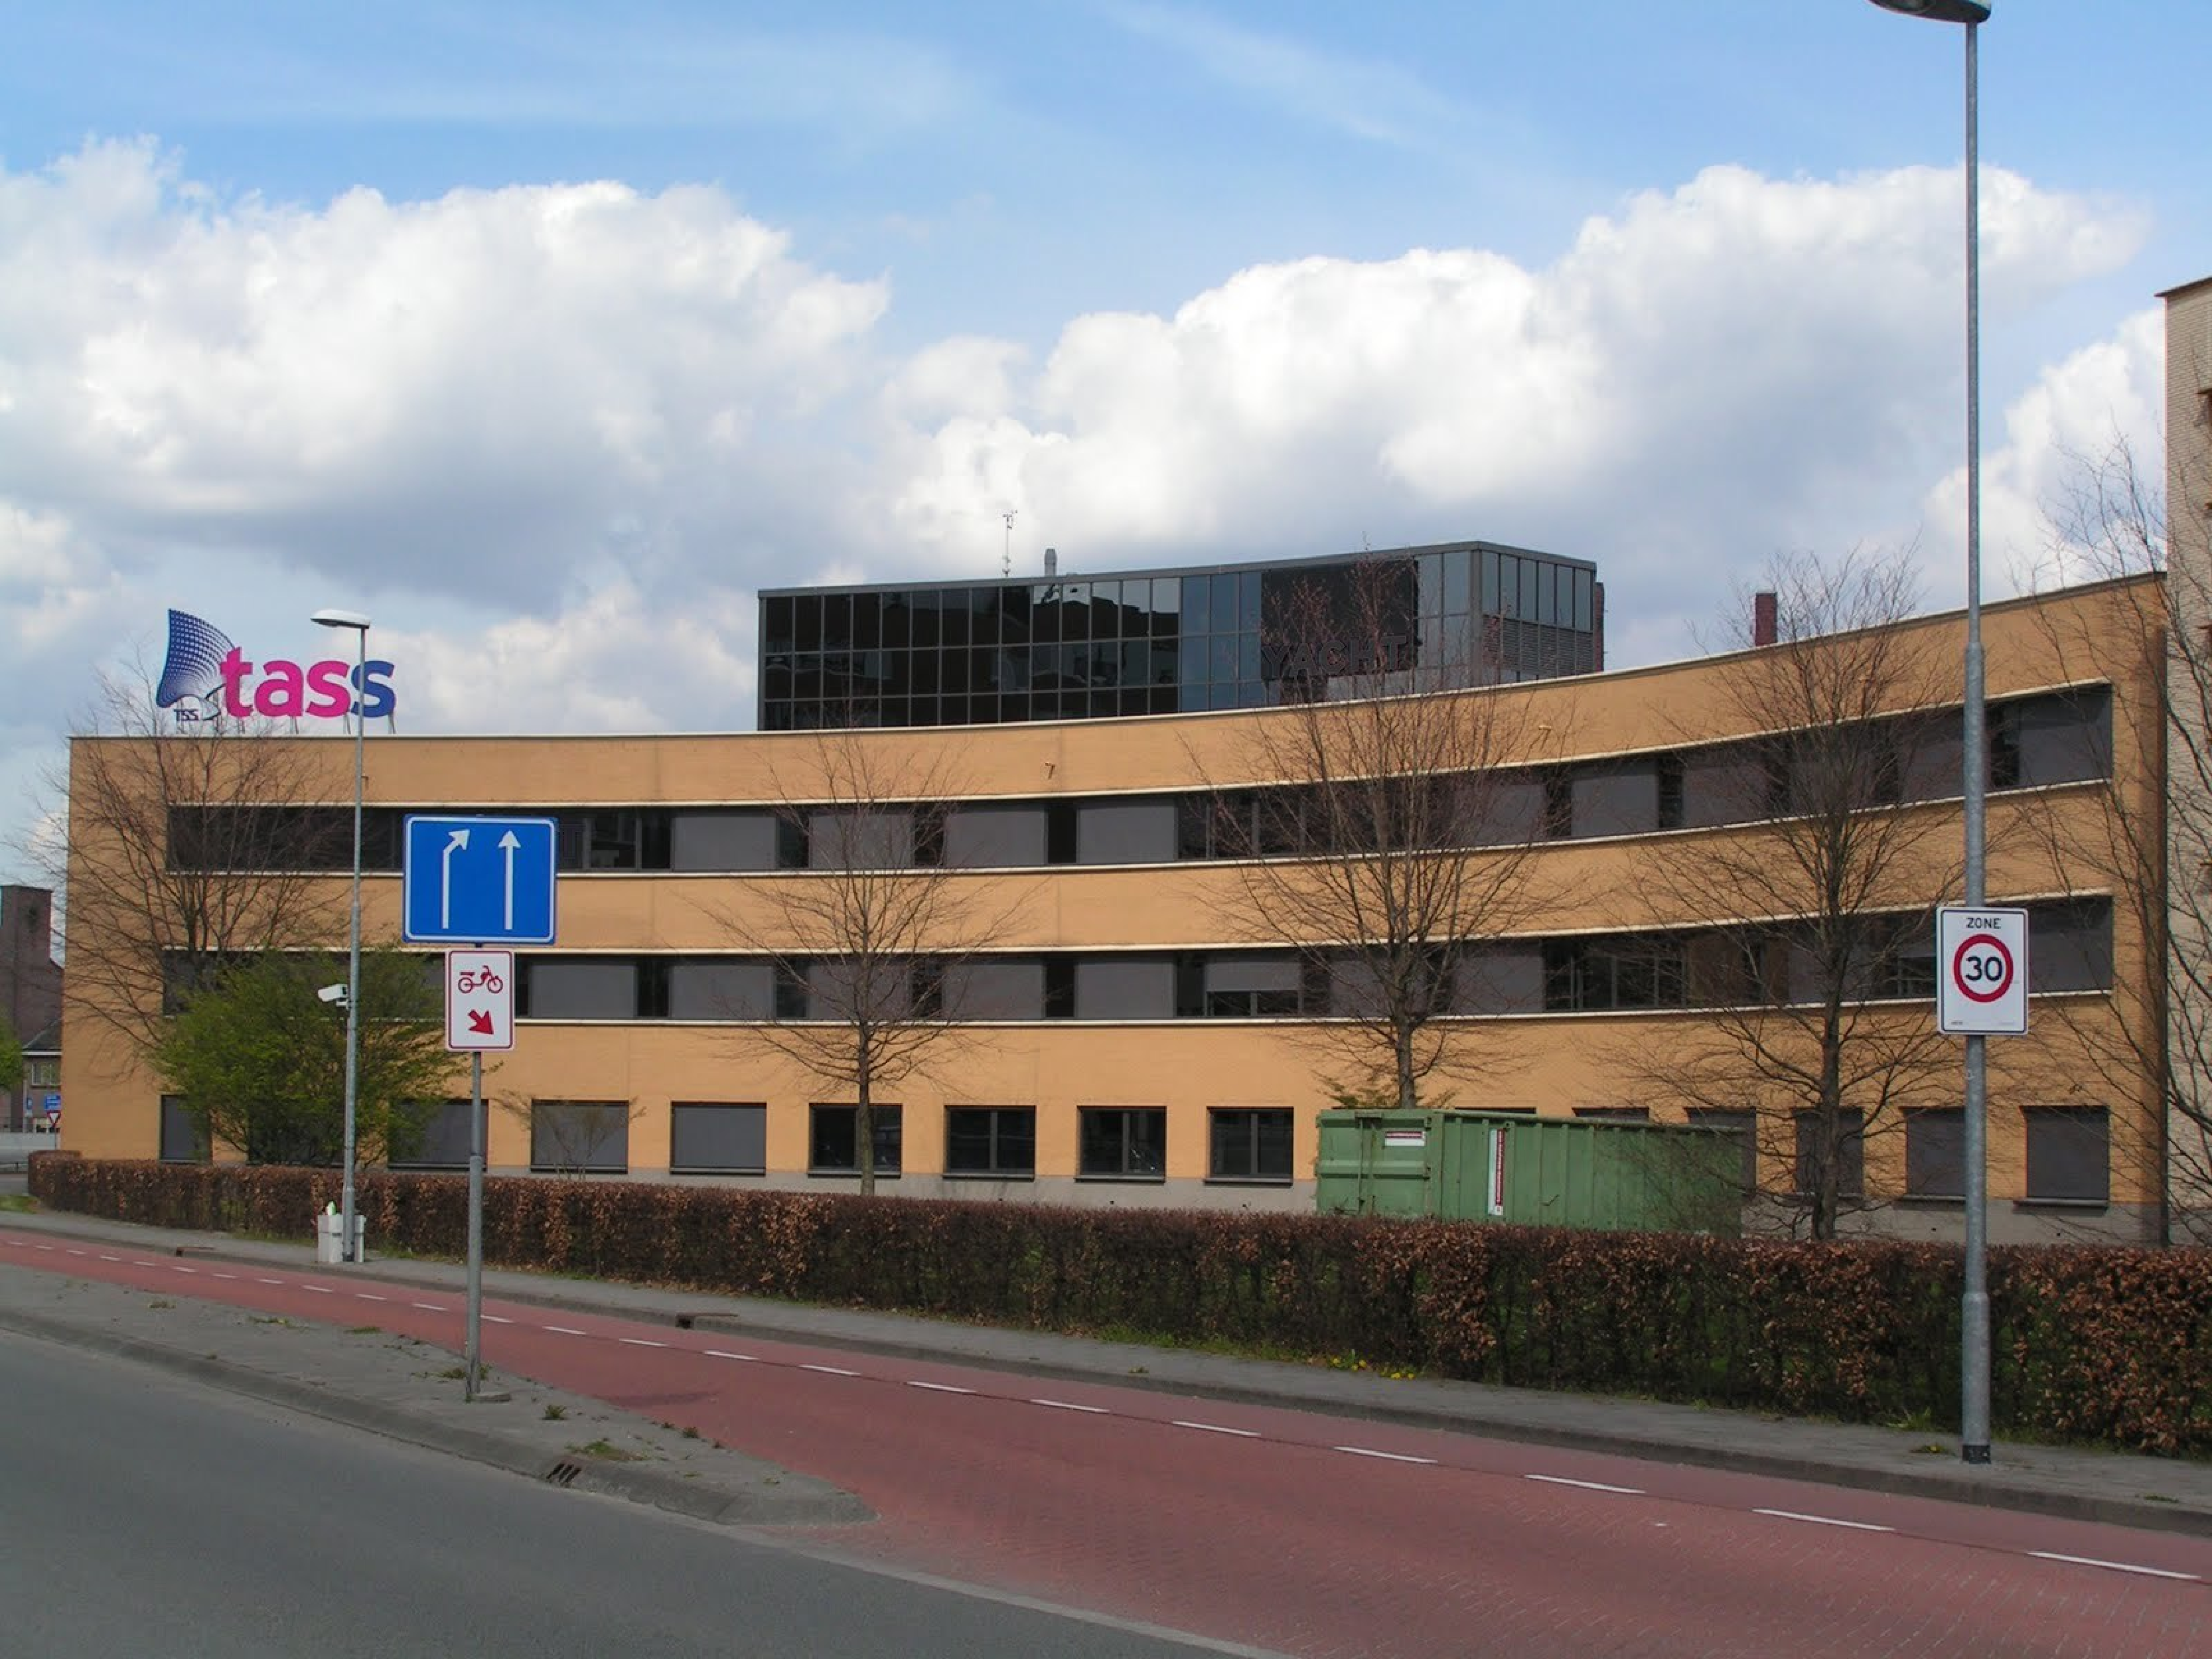
\includegraphics[width=0.40\textwidth]{tass_eindhoven.pdf}
  \end{center}
  \caption{TASS Eindhoven}
\end{wrapfigure}

TASS is een detacheringsbedrijf wat betekent dat het personeel werkzaam is bij
andere bedrijven. Zeker gezien hun geschiedenis heeft TASS nog een goede
relatie met het vroegere moederbedrijf Philips en werkt dus ook veel met Philips
samen. Andere bedrijven waar veel mee wordt samengewerkt zijn TomTom, ASML
en Bosch.

Naast het detacheren heeft TASS ook een aantal projecten intern lopen. Het
grootste en meest bekende project is het uCAN project. Dit project
focust zich op het inzichtelijk maken van sensorgegevens uit auto's. uCan
leest de CAN-Bus uit en zendt de informatie door naar een server in de
cloud.

Binnen TASS is het grootste deel van het personeel gedetacheerd bij andere
bedrijven. Deze medewerkers krijgen allemaal een people manager toegewezen.
Deze people manager zorgt voor de relatie tussen TASS en de medewerker evenals
het helpen van oplossen van eventuele problemen tussen de medewerker en het bedrijf waar deze
gedetacheerd zit.

De plek waar de medewerker gedetacheerd is, wordt geregeld door de account
managers van TASS. Een account manager heeft een aantal bedrijven in
zijn/haar portfolio zitten met wie ze contact hebben over mogelijke
opdrachten voor medewerkers. Mochten ze een plek vinden, zorgen zij voor
een goede kandidaat in samenwerking met de people managers.

Tijdens het afstuderen is er voor de studenten ook een people manager
die het project zal begeleiden, in dit geval is dat Gerben Blom. Deze
people manager zal de afstudeerders begeleiden op projectmatig vlak,
functioneren als Project Owner en eventueel antwoord geven op technische
vragen.

Tweewekelijks zal er een review punt komen waar de people manager
samenkomt met de afstudeerder om de voortgang en problemen te bespreken.
Tevens zal daar besproken en getoond worden wat voor producten er in die twee weken
opgeleverd zijn. Hierna zullen ook de taken van de komende twee weken
bepaald worden.

Buiten de People Manager krijgen de afstudeerders ook een technische
begeleider toegewezen. De hoofd technische begeleider heet Bas Burgers,
maar ook Berry Borgers is erg ge\"interesseerd is het DomoTop project en hij
wil graag de tweede technische begeleider zijn. De people manager is
niet meer dagelijks bezig met technische ontwikkeling en kan op dat vlak
eventueel achter lopen. Bas Burgers is een gedetacheerde medewerker, die zich nog
dagelijks bezighoudt met de techniek.
Deze technische begeleider zal zich dan ook niet bezig houden met 
project management zaken, maar vooral met de technische problemen of vragen
project management zaken maar vooral met de technische problemen of vragen
waar tegenaan gelopen wordt.

De klant zal in dit project vertegenwoordigd worden door de People Manager
Gerben Blom. Hij zal in dit project niet de enige klant zijn, ook de
ontwikkelaars en gebruikers van het OpenRemote project zullen de rol van klant
op zich nemen. Dit betekent dat de documentatie van het project hierop aangepast
moet worden, er zal moeten worden gedocumenteerd in het Engels.  
Het eindresultaat wordt gestuurd naar OpenRemote om op deze wijze de beveiliging
van OpenRemote te verbeteren. Daarom moet het project aan de standaarden voldoen die OpenRemote stelt. 
De keuzes moeten verantwoord kunnen worden richting de ontwikkelaars van
OpenRemote. Tevens kunnen de ontwikkelaars van OpenRemote bij het DomoTop project helpen en deze begeleiden.

Tot slot zijn de afdelingen HR en ICT beheer bij het project betrokken. Bij
de HR afdeling worden zaken als contracten behandeld. Bij de ICT beheer
afdeling binnen de organisatie moet er gedacht worden aan het bestellen van
hardware en het opzetten van computers. Ook bij computer gerelateerde problemen of
bij vragen kan men bij deze afdeling terecht.

\newpage
\section{Probleemanalyse}
Binnen de opdracht is een probleemsituatie onstaan die hieronder
beschreven worden. Naar aanleiding van deze probleemsituatie is er een
probleemstelling opgesteld.

\subsection{Probleemsituatie}

Het open source domotica platform OpenRemote is een software pakket dat
gebruikers in staat stelt een domotica systeem op te zetten in huis dat
overweg kan met meerdere domotica protocollen. Dit systeem bestaat uit drie
delen, ten eerste de OpenRemote controller. Deze controller is een stuk
software dat draait op een computer binnen het huis dat door middel van
domotica geautomatiseerd kan worden.

De controller communiceert rechtstreeks met het tweede onderdeel van het
OpenRemote pakket, namelijk de client applicatie. Er is een Android, iOS en
webapplicatie te downloaden die kan werken met de OpenRemote controller.

De gebruikersinterface van deze applicaties wordt, samen met de logica
erachter, ontworpen via het derde onderdeel: de composer. Deze composer is
een web applicatie die de mogelijkheid geeft tot het ontwerpen van de
client applicatie, evenals het configureren van de actie of acties die
gebeuren als er bijvoorbeeld een knop wordt ingedrukt.

Dit software pakket heeft echter een groot gebrek, het is niet beveiligd
afgezien van een globale gebruikersnaam en wachtwoord voor het hele
systeem. Dit is niet gewenst en deze opdracht is bedoeld om dit te verhelpen door
er een authenticatie en autorisatie mechanisme aan toe te voegen.

\subsection{Probleemstelling}

Het probleem dat opgelost moet worden is dat onbevoegden makkelijk toegang
kunnen krijgen tot een OpenRemote systeem. Voor dit probleem is de
volgende doelstelling geformuleerd: het implementeren van beveiliging in
OpenRemote, zodat onbevoegden geen toegang kunnen krijgen tot het systeem.

Het eerste deelprobleem dat is te defini\"eren over deze probleemstelling is:
Welke beveiligingstechnieken zijn het best te gebruiken in deze situatie?
Deze doelstelling zal onderzocht worden en uiteindelijk ge\"implementeerd worden
in OpenRemote.

Het tweede deelprobleem dat opgelost moet worden is: De ontwikkelaars
moeten de code van OpenRemote doorgronden om deze uiteindelijk uit te
kunnen breiden. Voordat er aan de slag kan worden gaan met uitbreiding van
OpenRemote moet de code eerst onderzocht worden.

De volgende probleemstelling die opgelost moet worden binnen het project
is: geselecteerde gebruikers moet toestemming tot het systeem kunnen worden
verleend. Deze probleemstelling gaat meer richting de autorisatie en over
hoe men gebruikers toestemming kan geven tot een systeem.

Het laatste probleem dat gedefinieerd is: er kunnen groepen gemaakt worden om
rechten aan gebruikers te geven, zodat knoppen alleen toegankelijk zijn voor een
deel van de gebruikers. 

Voor dit project is SCRUM gebruikt als ontwikkelmethodiek, mede omdat het een
zeer flexibele ontwikkelmethode is voor het ontwikkelen van software. Zo is het
mogelijk met SCRUM om, zonder dat alle eisen bekend zijn, meerdere tussenopleveringen te hebben, 
wat de kwaliteit ten goede komt. Voor meer
informatie zie het hoofdstuk 'Methoden en Technieken'.

\newpage
\section{Plan van Aanpak}

In dit hoofdstuk wordt er een samenvatting gegeven van het plan van aanpak.  Zie
voor het volledige plan van aanpak bijlage 1. Het doel van het project is
OpenRemote  te  beveiligen  en  dit  eventueel  te demonstreren. Op dit moment
is er geen enkele manier van beveiliging aanwezig in OpenRemote. Ook zal er
gebruik gemaakt worden van een PlugTop, waarop  de OpenRemote server komt te
draaien.

Er zal gebruik gemaakt worden van  SCRUM, een ontwikkelmethode, welke flexibel
is en resulteert in een product dat  veel meer aan de verwachtingen van de klant
voldoet. Meer informatie  over  SCRUM kan gevonden worden in het hoofdstuk
'Methoden en technieken'.  Git wordt gebruikt als versiebeheer software en
dat  in  combinatie  met GitHub, waar de git hosting online geregeld is.  Er
zal  Google  Documenten gebruikt worden, waarin de documenten geschreven en
opgeslagen worden.  Al deze technieken komen ook verder aan bod in het
hoofdstuk  'Methoden  en technieken'.

In de eerste weken wordt  er  onderzoek  gedaan  naar  welke  technieken  er
gebruikt gaan worden. Welk platform,  PlugTop (een kleine computer server voor
gebruik in huis / kantoor)  en  protocollen  er  gebruikt gaan worden. Daarna
wordt de PlugTop opgezet samen met een  mobiel  apparaat (Android)  waarop
OpenRemote  draait. Er wordt een 'Research  Security' document opgezet. Hierin
komt een conclusie te staan wat de aanpak wordt  om OpenRemote het beste  te
beveiligen.  Met  deze  informatie  wordt  er  een prototype ontwikkeld. Nadat
er een volledig werkend  prototype  is,  kan  er gekeken worden of en waar dit
product uitgebreid en verbeterd kan worden.

Zie bijlage 1 voor het volledige plan van aanpak met daarin een lijst  van
risico's,  afspraken,  deadlines  en  een weekplanning.

\newpage
\section{Methoden en Technieken}

Binnen het project zijn er een aantal methoden, technieken en tools
gebruikt om het project tot een goed einde te brengen. Hier zullen de
verschillende keuzes voor methoden, technieken en tools toegelicht worden.

\subsection{Ontwikkelmethodiek}
De eerste keuze was voor een ontwikkelmethodiek. De ontwikkelmethodiek
moest een duidelijke voortgang kunnen laten zien door het project heen. De
begeleider vanuit school moet goed op de hoogte gehouden kunnen worden van
de voortgang, evenals de bedrijfsbegeleider. SCRUM is, met de review
momenten, hier een geschikte techniek voor doordat er bij elke SCRUM meeting de
resulaten worden besproken en er notulen van gemaakt worden. Deze notulen worden
overhandigd aan de schoolbegeleider. Tevens is binnen het bedrijf veel
kennis en expertise over SCRUM aanwezig, dus kan de methodiek ondersteund worden
vanuit het bedrijf.

\begin{figure}[htpb]
  \begin{center}
    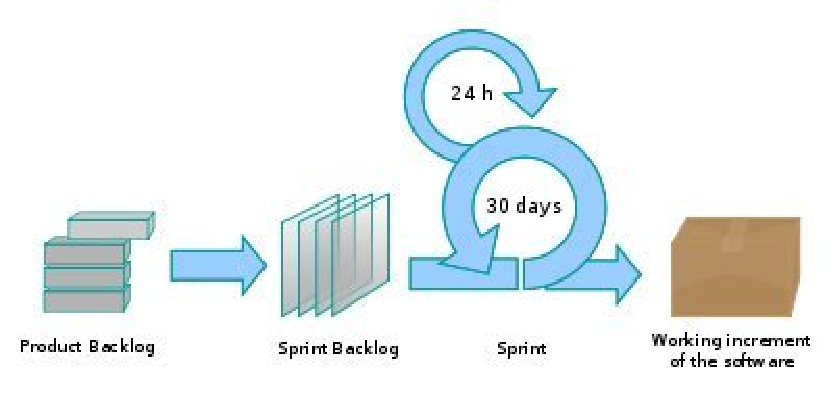
\includegraphics[width=0.80\textwidth]{scrum.pdf}
  \end{center}
  \caption{Scrum}
\end{figure}

TASS heeft een interne website opgezet, genaamd Sensei, waarin
veel informatie over SCRUM is opgenomen. Tevens zijn er een
aantal personen binnen het bedrijf SCRUM-experts, wat betekent dat vragen of
problemen altijd beantwoord kunnen worden door een van de experts.

Voor de verschillende SCRUM backlogs is ervoor gekozen een spreadsheet te
gebruiken. Er is gekeken naar verschillende software oplossingen, maar geen
voldeed aan de verwachtigingen. Een eigen spreadsheet heeft veel
flexibiliteit, alles wat er nodig zou kunnen zijn kan zelf ingebouwd worden.

Tevens zijn er meerdere burndown charts om de voortgang snel in te kunnen
zien en bij te kunnen houden. Deze burndown charts houden verschillende
elementen van de backlogs bij om op deze manier alles inzichtelijk te
houden.

\newpage
\subsection{Versiebeheer}

De techniek die gebruikt wordt om code en documentversies bij te houden is
git. Git is een 'version control system' net als subversion en
mercurial. Het doel van git is om verschillende versies van bestanden bij
te houden en te kunnen springen in versies. Git heeft als grote voordeel
dat het gedistribueerd is, wat betekent dat elke git clone (vergelijkbaar
met een svn checkout) een volledige geschiedenis met zich meebrengt. Het is
dus niet noodzakelijk een centrale server te gebruiken, al wordt dit vaak
wel gedaan. Dat betekent ook dat elke git clone een backup is van de gehele
geschiedenis. Een ander voordeel van git is, dat er veranderingen opgeslagen
kunnen worden (commit) en later pas gedeeld worden met andere mensen (push). Dit in
tegenstelling tot andere versies beheersystemen waarbij deze functinaliteit niet
aanwezig is. Zie de werking en belangrijke commando's van git in figuur \ref{git}.

\begin{figure}[htpb]
  \begin{center}
    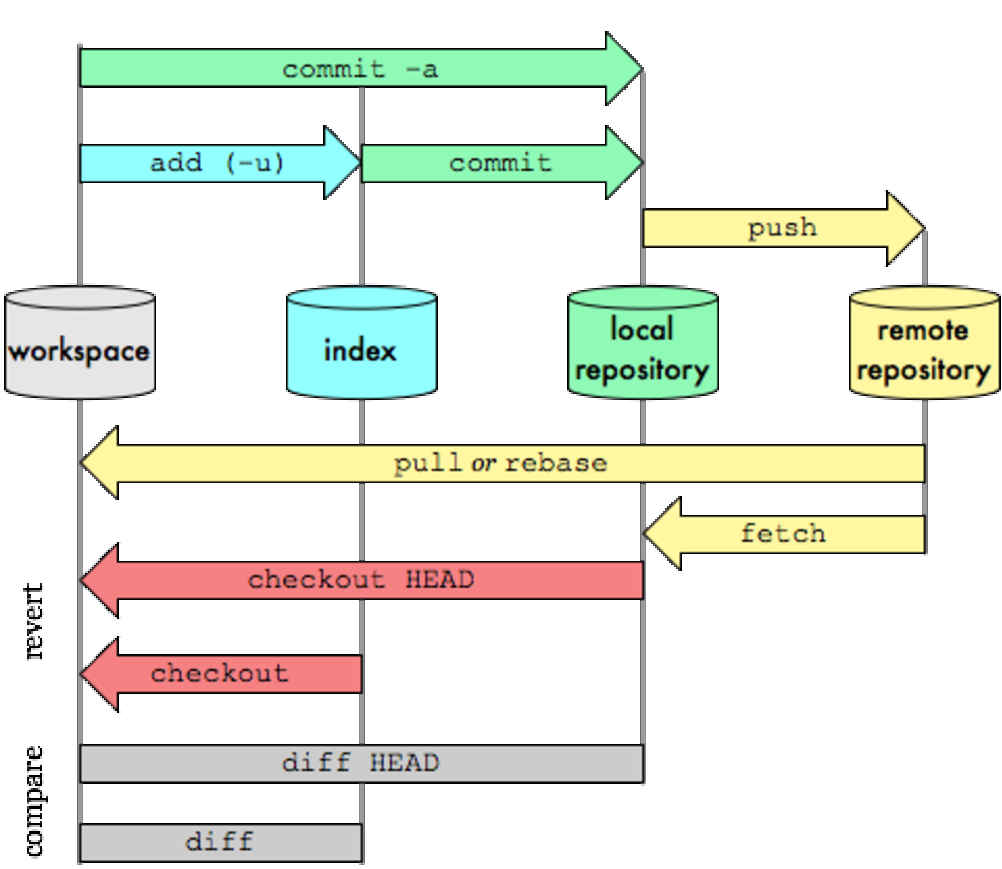
\includegraphics[width=0.50\textwidth]{git_diagram.pdf}
  \end{center}
  \caption{Werking git}
  \label{git}
\end{figure}

Om toch een centrale plaats te hebben waar alle veranderingen naartoe
gestuurd worden, hebben wij ervoor gekozen om Github te gebruiken. Github
is een online platform voor git-repositories, met een erg goede
webinterface. In deze webinterface kan de code bekeken worden. Tevens kan de git url
gevonden worden en kunnen 'issues' aangemaakt worden.

\subsection{Testen}
Testen zorgt voor hogere kwaliteit van de
software. Standaard zijn er in OpenRemote al unit-tests aanwezig. Omdat de
gemaakte software gefocust is op beveiliging, is er gekozen om verschillende
penetratietesten uit te laten voeren. Er is een student aanwezig binnen het bedrijf, die hier al meer
kennis en ervaring heeft met penetratietesten. Deze persoon heeft verschillende keren een
penetratietest uitgevoerd met als doel binnen te komen in het systeem zonder
identificatie, authenticatie en/of autorisatie. Veiligheidslekken die gevonden
worden, zijn direct opgelost en later opnieuw getest of het daadwerkelijk is
opgelost.

\subsection{Documenten}
Voor het maken van documenten is gekozen voor Google Documenten.
Google Documenten is een web applicatie waarmee eenvoudig en
snel documenten kunnen worden gemaakt. Tevens is het mogelijk om met
meerdere mensen in een document te werken zonder conflicten te krijgen. Ook
de SCRUM spreadsheets staan in Google Documenten.

Voor het afstudeerverslag is er gekozen voor \LaTeX. Dit omdat het opmaken
van een document veel meer mogelijkheden met zich meebrengt dan het meer
beperkte Google Documents. Ook bestond de wens bij studenten
om meer ervaring op te doen met \LaTeX\space. Het afstudeerverslag leek hen een uitgelezen kans hiervoor.

\subsection{Programmeertalen}
De talen die gebruikt gaan worden liggen al vast, aangezien er verder 
gewerkt wordt op een bestaand project. Voor de controller wordt gebruik gemaakt van
Java, evenals voor de composer en beehive. De verschillende applicaties maken gebruik
van Java op Android en Objective-C op iOS.

\subsection{Database}
Er is gebruik gemaakt van RazorSQL. Met dit programma is het mogelijk om
SQL queries op te zetten, uit te voeren en te testen via een grafische
interface. RazorSQL werkt ook met de database die gebruikt wordt bij het DomoTop project,
genaamd HSQLDB. In deze database worden gegevens opgeslagen van de
apparaten die zich aanmelden bij OpenRemote en bij de groepen.
RazorSQL is enkel een tool die gebruikt is bij het
testen/opzetten van de database, daarom is deze tool niet meer
noodzakelijk.

Er is gekozen voor HSQLDB vanwege het feit dat deze database 100\% in Java
is geschreven (net als de Controller van OpenRemote), volledig open-source is,
relatief weinig impact heeft op het systeem en multithreaded is.
HSQLDB is namelijk klein en gebruikt weinig bronnen van het systeem. Tot slot voldoet
HSQLDB aan alle eisen en beschikt over alle mogelijkheden die noodzakelijk
zijn binnen het DomoTop project. Denk hierbij aan tabellen aanmaken, rijen
toevoegen, updaten, verwijderen en nog veel meer. Alternatieven van HSQLDB zijn
niet in native Java geschreven. Deze vragen meer van het systeem qua
bronnen en zijn groter dan HSQLDB. Sommige alternatieven zijn zelfs niet
eens geschikt om te gebruiken in combinatie met een TomCat server.

\subsection{Ontwikkelomgeving}
Voor de Android applicatie wordt gebruik gemaakt van de Eclipse
ontwikkelomgeving met de ADT plugin. Hiermee is het makkelijk om wijzigingen
live te draaien op een tablet of een emulator.

Bij het programmeren van de OpenRemote Controller wordt er ook gebruik gemaakt
van de Eclipse omgeving. OpenRemote Controller is in Java geschreven code
en deze Controller is ook vanaf het begin af aan gestart in de Eclipse
ontwikkelomgeving. Omdat OpenRemote Controller al ontwikkeld is in
Eclipse, wordt er ook gebruik gemaakt van Eclipse. Er wordt gebruik gemaakt van Ant 
om de Controller te bouwen en te compileren. Uiteindelijk krijg
je \'e\'en WAR bestand. Deze WAR kan eenvoudig ge\"importeerd worden in de TomCat
Web Application Manager, waarna de Controller gebruikt kan worden. TomCat is
de webserver die OpenRemote al gebruikt om de OpenRemote Controller op te
kunnen zetten. Het DomoTop project heeft daarom ook TomCat gebruikt, omdat
dit de meest toegankelijke oplossing is, gezien het feit dat OpenRemote hier
ook al mee werkt.

Tevens wordt gebruik gemaakt van een Eclipse plugin genaamd Colorer.
Met deze plugin is het mogelijk om syntax highlighting aan te zetten voor
XML/HTML documenten, maar ook CSS en JavaScript bestanden. Er is hiervoor
gekozen, omdat Eclipse standaard geen highlighting heeft voor bovengenoemde
type bestanden. Desalniettemin is het optioneel om de Eclipse Colorer
plugin te gebruiken. Het is enkel gekozen om optimaler te kunnen ontwikkelen.

\subsection{Libraries}
\begin{figure}[htpb]
   \begin{center}
     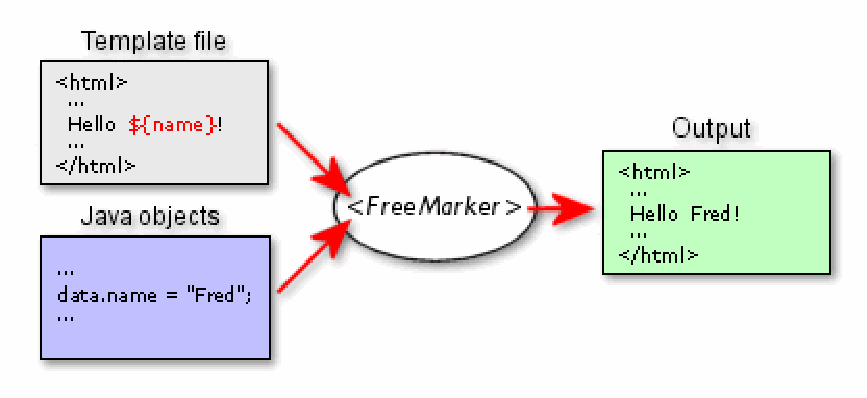
\includegraphics[width=0.6\textwidth]{freemarker.pdf}
   \end{center}
   \caption{FreeMarker}
\end{figure}

In de OpenRemote Controller is er gebruikt gemaakt van een template engine
genaamd Freemarker. Deze template engine maakt het mogelijk om statische
opmaak (template design) te scheiden van dynamische gegevens, zoals apparaatgegevens
uit een database. Freemarker werkt goed samen met Java en TomCat.
Verder is FreeMaker een relatief kleine template engine en simpel te
begrijpen maar toch doeltreffend. FreeMarker forceert het gebruik
van een Model View Controller software architectuur. FreeMarker wordt ook
vaak gebruikt voor servlet gebaseerde web applicatie ontwikkeling, en dat is
exact wat de OpenRemote Controller is.

Om te kunnen werken met encryptie en TLS in native Java code, wordt er gebruik
gemaakt van Bouncy Castle wat gratis open source software is.  Bouncy Castle is
een bibliotheek die binnen het project gebruikt wordt om onder andere nieuwe
certificaten te kunnen genereren vanuit Java code. Ook kan deze bibliotheek een
CSR (Certificate Signing Request) bestand uit lezen en deze gegevens te
gebruiken om een nieuw certificaat te ondertekenen door middel van een CA
(Certificate Authority). In dit CSR bestand staat onder andere de publieke
sleutel van de aanvrager alsmede extra informatie over de persoon die het
certificaat probeert aan te vragen.  Certificate Authority beheert alle
certificaten. Zie de begrippenlijst voor meer informatie. Ook het gebruikte CA
certificaat wordt aangemaakt door middel van Bouncy Castle. Onder Android wordt
er ook gebruik gemaakt van de Bouncy Castle bibliotheek, echter heet dat onder
Android Spongy Castle, maar het is exact dezelfde code.

\newpage
\begin{wrapfigure}{R}{0.25\textwidth}
  \begin{center}
    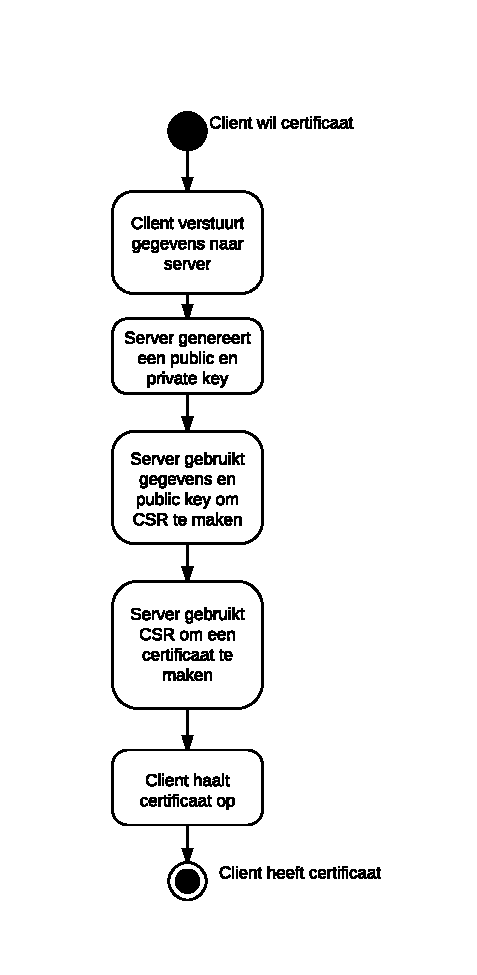
\includegraphics[height=0.70\textheight]{ssl_ad_1.pdf}
  \end{center}
  \caption{SSL workflow}
  \label{ssl_ad_1}
\end{wrapfigure}
\section{Uitvoering}

\subsection{Onderzoek}

Het begin van de stage stond in het teken van onderzoek. Er was bij het
ontwikkelteam weinig kennis van het domotica veld, OpenRemote, PlugTop computers
en beveiliging, dus al deze velden moesten onderzocht worden. Het project begon
met een globaal onderzoek naar het domotica domein en naar PlugTop computers. Het
volgende onderzoek dat uitgevoerd werd, was naar het OpenRemote software pakket en
eventuele alternatieven.

Het laatste onderzoek is gedaan naar de beveiligingstechnieken die bestaan.
Voorafgaan aan het onderzoek is er gesproken met Berry Borgers
aangezien hij over veel kennis beschikt met betrekking tot beveiling. De keuzes
die zijn gemaakt in het document zijn in overleg met Berry Borgers gebeurd. Dit
onderzoek is gedocumenteerd in het Engels zodat het te delen is met de
ontwikkelaars van OpenRemote. Alle onderzoeken zijn  te vinden in de bijlagen.

\subsection{TLS}
Vervolgens is er begonnen met het ontwikkelen van de gekozen oplossing:
TLS implementeren in OpenRemote om deze veiliger te maken. Dit gebeurt
door een apparaat een aanvraag te laten doen bij de OpenRemote Controller. De
OpenRemote Controller kan deze aanvraag goedkeuren en het apparaat ontvangt
vervolgens het client certificaat. Dit client certificaat wordt vervolgens
gebruikt in combinatie met een apparaat (zoals Android), waarna er toestemming
wordt verleend om de OpenRemote Controller te gebruiken.

De client heeft een certificaat nodig om een veilige verbinding op te kunnen
zetten met de server. Met dit certificaat kan een client zich identificeren en
authenticeren bij een server. Een certificaat wordt gegenereerd op de manier
zoals te zien in figuur \ref{ssl_ad_1}. In een certificaat moeten gegevens staan
waarmee de client te identificeren is. Als er een aanvraag wordt gedaan, moet de
beheerder kunnen zien van wie deze aanvraag komt. Er is in het project gekozen
om hiervoor de naam van het apparaat (tablet/telefoon) evenals het emailadres te
gebruiken. Hiervoor is gekozen omdat deze gegevens in de meeste apparaten
voorkomen en uit te lezen zijn. Met deze twee gegevens is het voor een beheerder
mogelijk  De client verzamelt deze gegevens en verstuurt deze naar de server. 

De server genereert voor de client een nieuw keypair, met daarin een
public en een private key. Vervolgens worden de public key en de gegevens van de
client gebruikt om een certificate signing request (CSR) te genereren. Een
CSR is een bestand met daarin al de gegevens die een certificate authority (CA)
nodig heeft om een certificaat te genereren. Vervolgens gebruikt dezelfde server
deze CSR om een certificaat te maken. Het certificaat wordt samen met de private
key opgeslagen in een keystore. De public key hoeft niet apart opgeslagen te
worden, deze staat immers in het certificaat. Deze keystore kan vervolgens
opgehaald worden door de client en gebruikt worden om een veilige verbinding op
te zetten.

Het certificaat van de client wordt, zonder private key, ook opgeslagen in de
truststore van TomCat. TomCat gebruikt deze truststore om te controleren of een
certificaat te vertrouwen is. Als een certificaat niet in de truststore staat
is deze niet te vertrouwen en wordt er geen veilige verbinding opgezet. 

Nadat dit ge\"implementeerd was ontstond echter een probleem. TomCat leest
namelijk de truststore tijdens het opstarten \'e\'en keer in. De certificaten
die na het opstarten van TomCat toegevoegd worden aan de truststore, worden dus
niet gebruikt. Dit betekent dat na het toevoegen van een client, TomCat
geherstart zou moeten worden.  \\Om dat probleem op te lossen, dat de TomCat
server niet telkens herstart hoeft te worden, is ervoor gekozen om een eigen
'self-signed' CA te gebruiken. Op deze manier hoeft alleen het certificaat van
de CA toegevoegd te worden aan de truststore van TomCat.  Zolang de client
certificaten ondertekend zijn door een CA certificaat uit de truststore wordt
deze vertrouwd. Als een client vertrouwd wordt, kan deze gebruik maken van de
OpenRemote Controller. Zie figuur \ref{init_controller} hoe de OpenRemote
Controller ge\"installeerd wordt.

\newpage

\begin{figure}[htpb]
   \begin{center}
     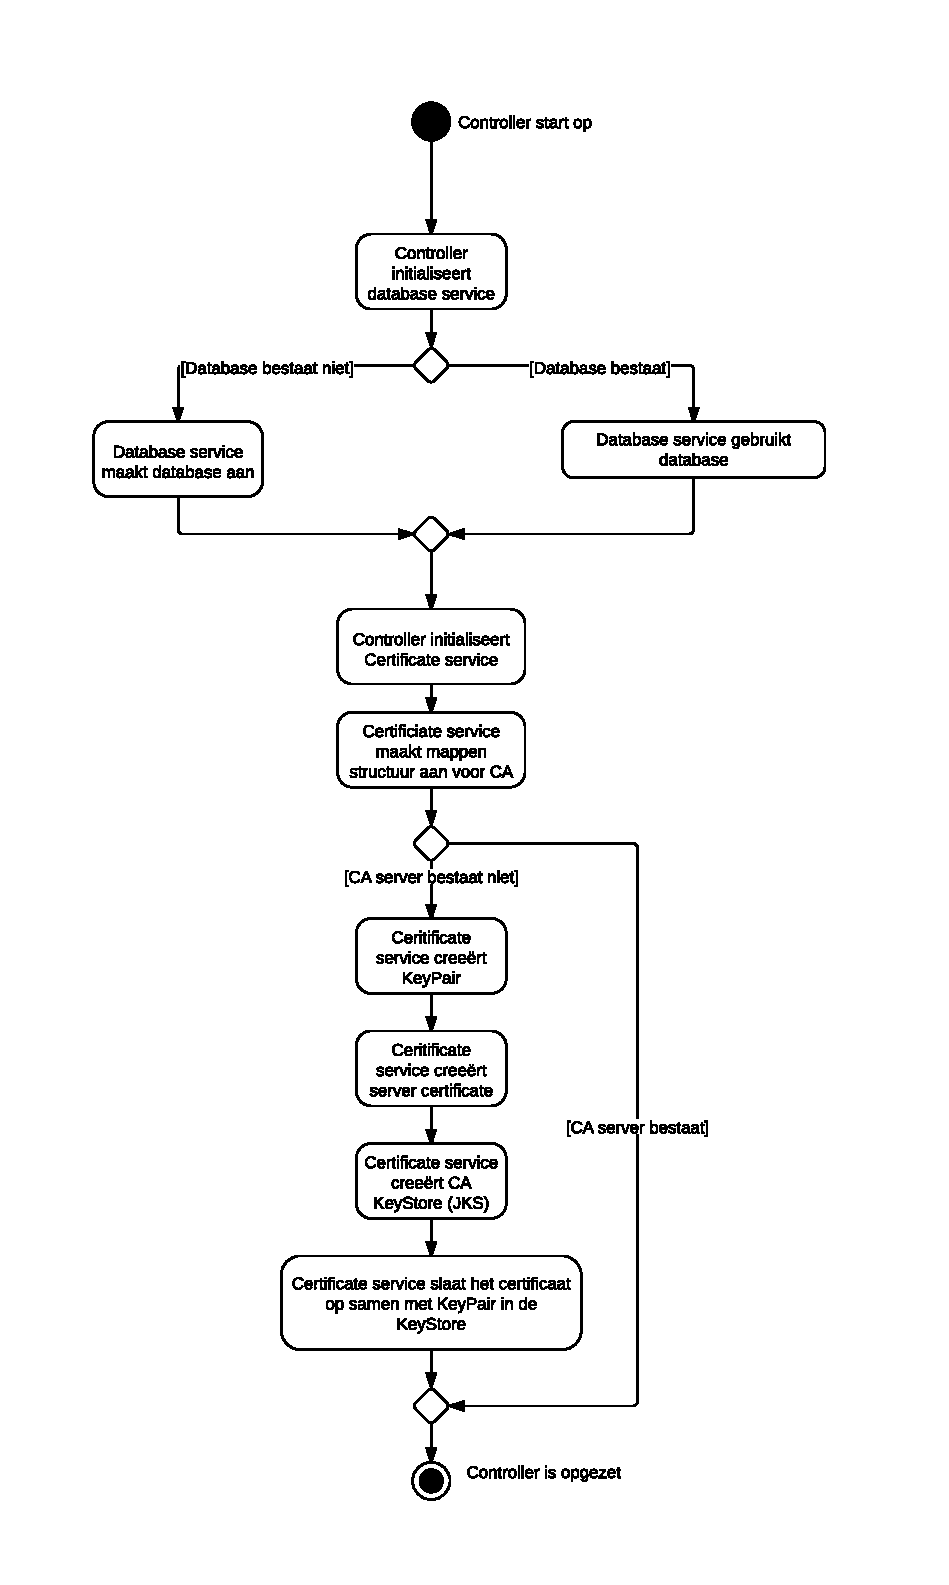
\includegraphics[height=0.84\textheight]{OpenremoteControllerAd.pdf}
   \end{center}
   \caption{Activity Diagram initalitatie OpenRemote Controller}
   \label{init_controller}
\end{figure}


Het oversturen van de client certificaten met de private key van server naar
client is een probleem. Mochten deze twee bestanden onderschept worden, kan een
ander apparaat deze gebruiken om een 'veilige' verbinding op te zetten. In het
ideale geval is het gewenst om het keypair en CSR op de client te genereren. De
CSR kan dan overgestuurd worden naar de server, waarna deze er een certificaat
van kan maken en kan ophalen. Als een CSR of certificaat onderschept
wordt, vormt dit geen probleem. Deze bestanden zijn public en mogen door
iedereen bekeken worden. De workflow is dan ook aangepast zoals te zien in
figuur \ref{ssl_ad_2}.

De client controleert eerst of er een certificaat aanwezig is voor de
desbetreffende server. Als deze aanwezig is, wordt het proces meteen gestopt en
kan er direct een veilige verbinding opgezet worden. Mocht er geen certificaat
zijn, wordt er gecontroleerd of er een keypair aanwezig is. Een client heeft
\'e\'en keypair die gebruikt kan worden om meerdere certificaten te
cree\"eren. Mocht er geen keypair aanwezig zijn, dan wordt deze gegenereerd. Anders
kan er direct een CSR gegenereerd worden. Deze CSR wordt vervolgens opgestuurd
naar de server.

De CA op de server gebruikt deze CSR om een certificaat te cree\"eren. Dit
certificaat hoeft vervolgens niet toegevoegd te worden aan de truststore van
TomCat omdat het ondertekend is door een vertrouwde partij, namelijk de CA. Het
certificaat van de CA moet wel toegevoegd zijn aan de truststore van TomCat.

Het certificaat kan vervolgens door de client opgehaald worden en gebruikt
worden voor een veilige verbinding. Op deze manier is de private key nooit
verstuurd es zal deze altijd lokaal op de client blijven staan. 

\newpage

\begin{figure}[htpb]
   \begin{center}
     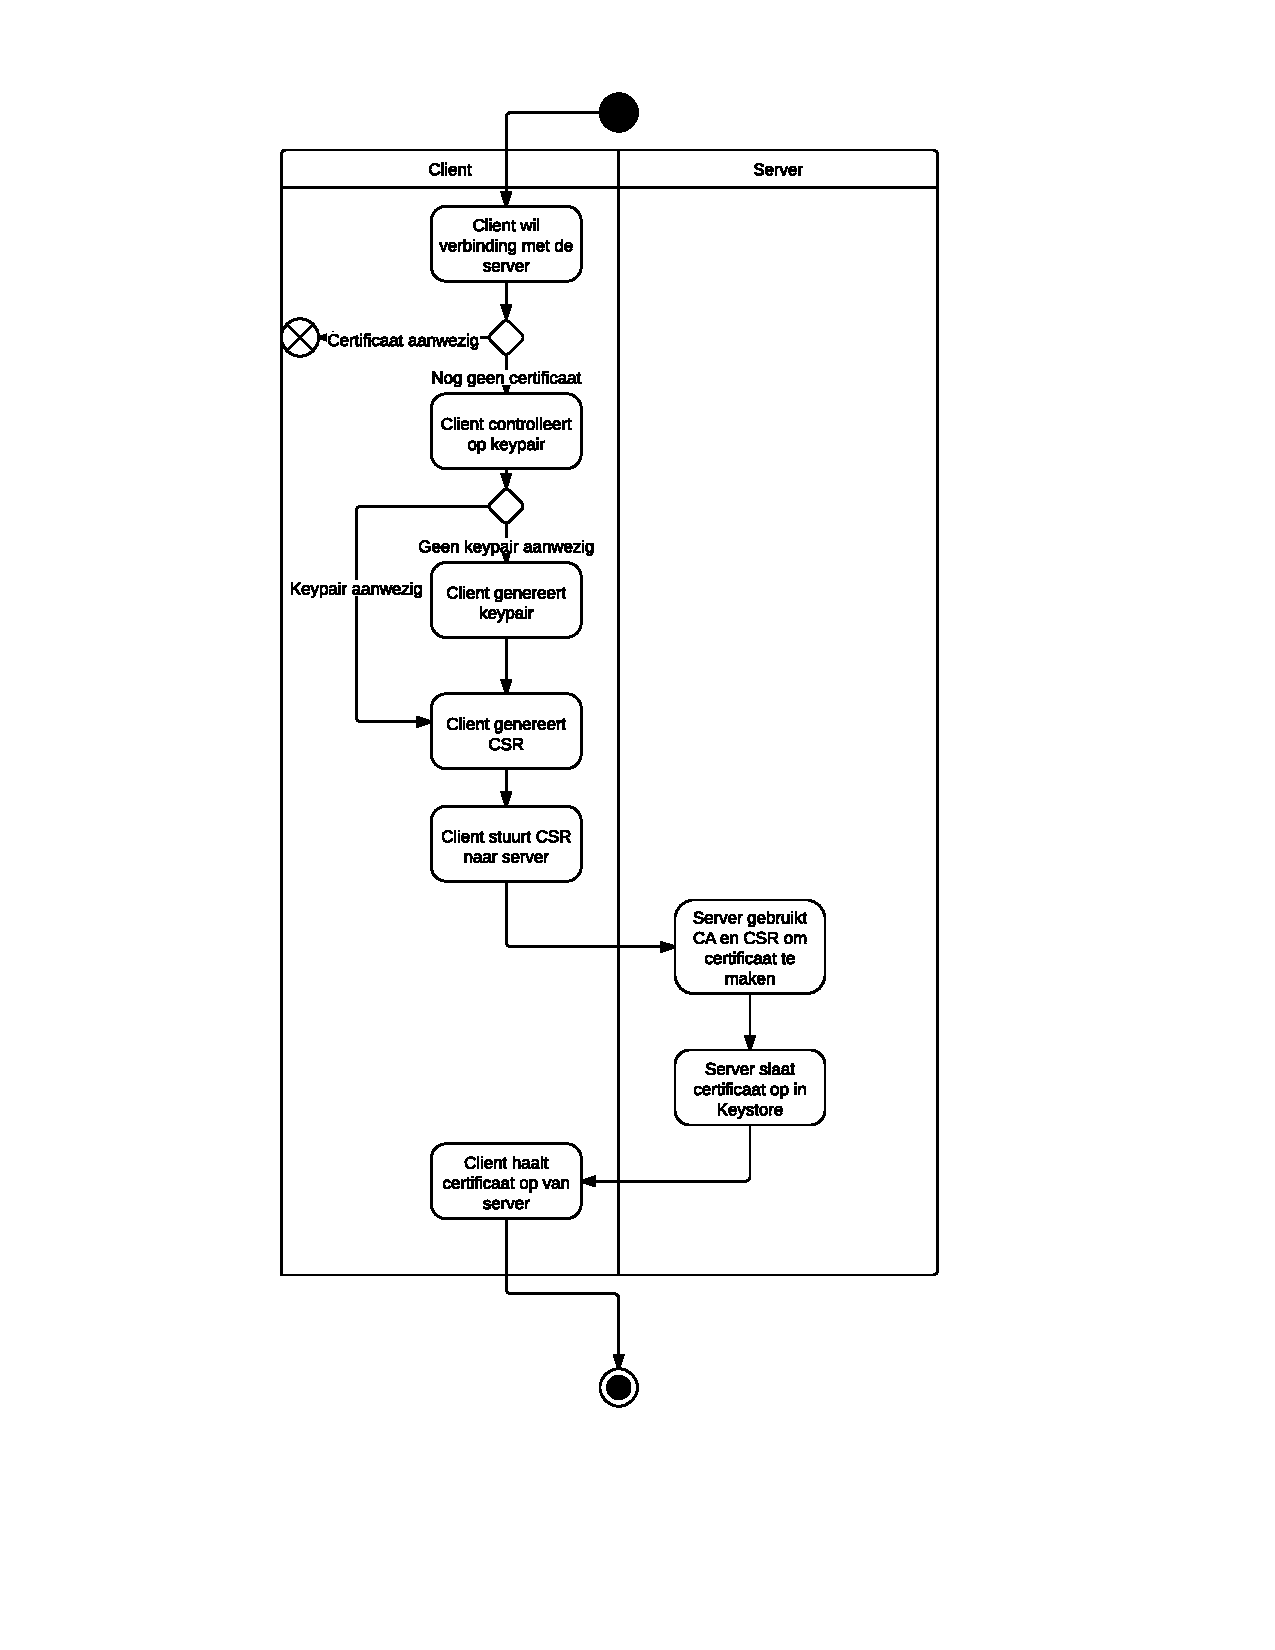
\includegraphics[height=0.86\textheight]{ssl_ad_2.pdf}
   \end{center}
   \caption{SSL workflow versie 2}
   \label{ssl_ad_2}
\end{figure}


\subsection{Android}
De client applicatie heeft als vereiste dat deze gegevens kan verzamelen. In het
begin om direct naar de server te sturen, later om zelf een CSR te sturen. De
naam van het apparaat zorgde niet voor problemen, echter het ophalen van het
emailadres wel. De app waar aan gewerkt is, is een bestaande app die al op de
market te vinden is. Deze app is beschikbaar voor android versies vanaf 1.5 en
hoger. Binnen het project moet er voor gezorgd worden dat deze app nog steeds
werkt met deze versie.

Om het emailadres op te halen wordt er gebruik gemaakt van de AccountManager van
Android. Deze is echter pas ge\"introduceerd in versie 2.1 van Android. Om dit
op te lossen is er gebruik gemaakt van reflection. Het ophalen van het
emailadres gebeurt met de AccountManager als de versie waar de app draait hoger
is dan 2.1. In lagere versies van Android geeft de app een standaard string
terug.

In de eerste versie van de app met certificaten is de interface veranderd. Er
zijn knoppen toegevoegd om de PIN op te vragen, een certificaat aan te vragen en
een certificaat op te halen.

\begin{figure}[htpb]
   \begin{center}
     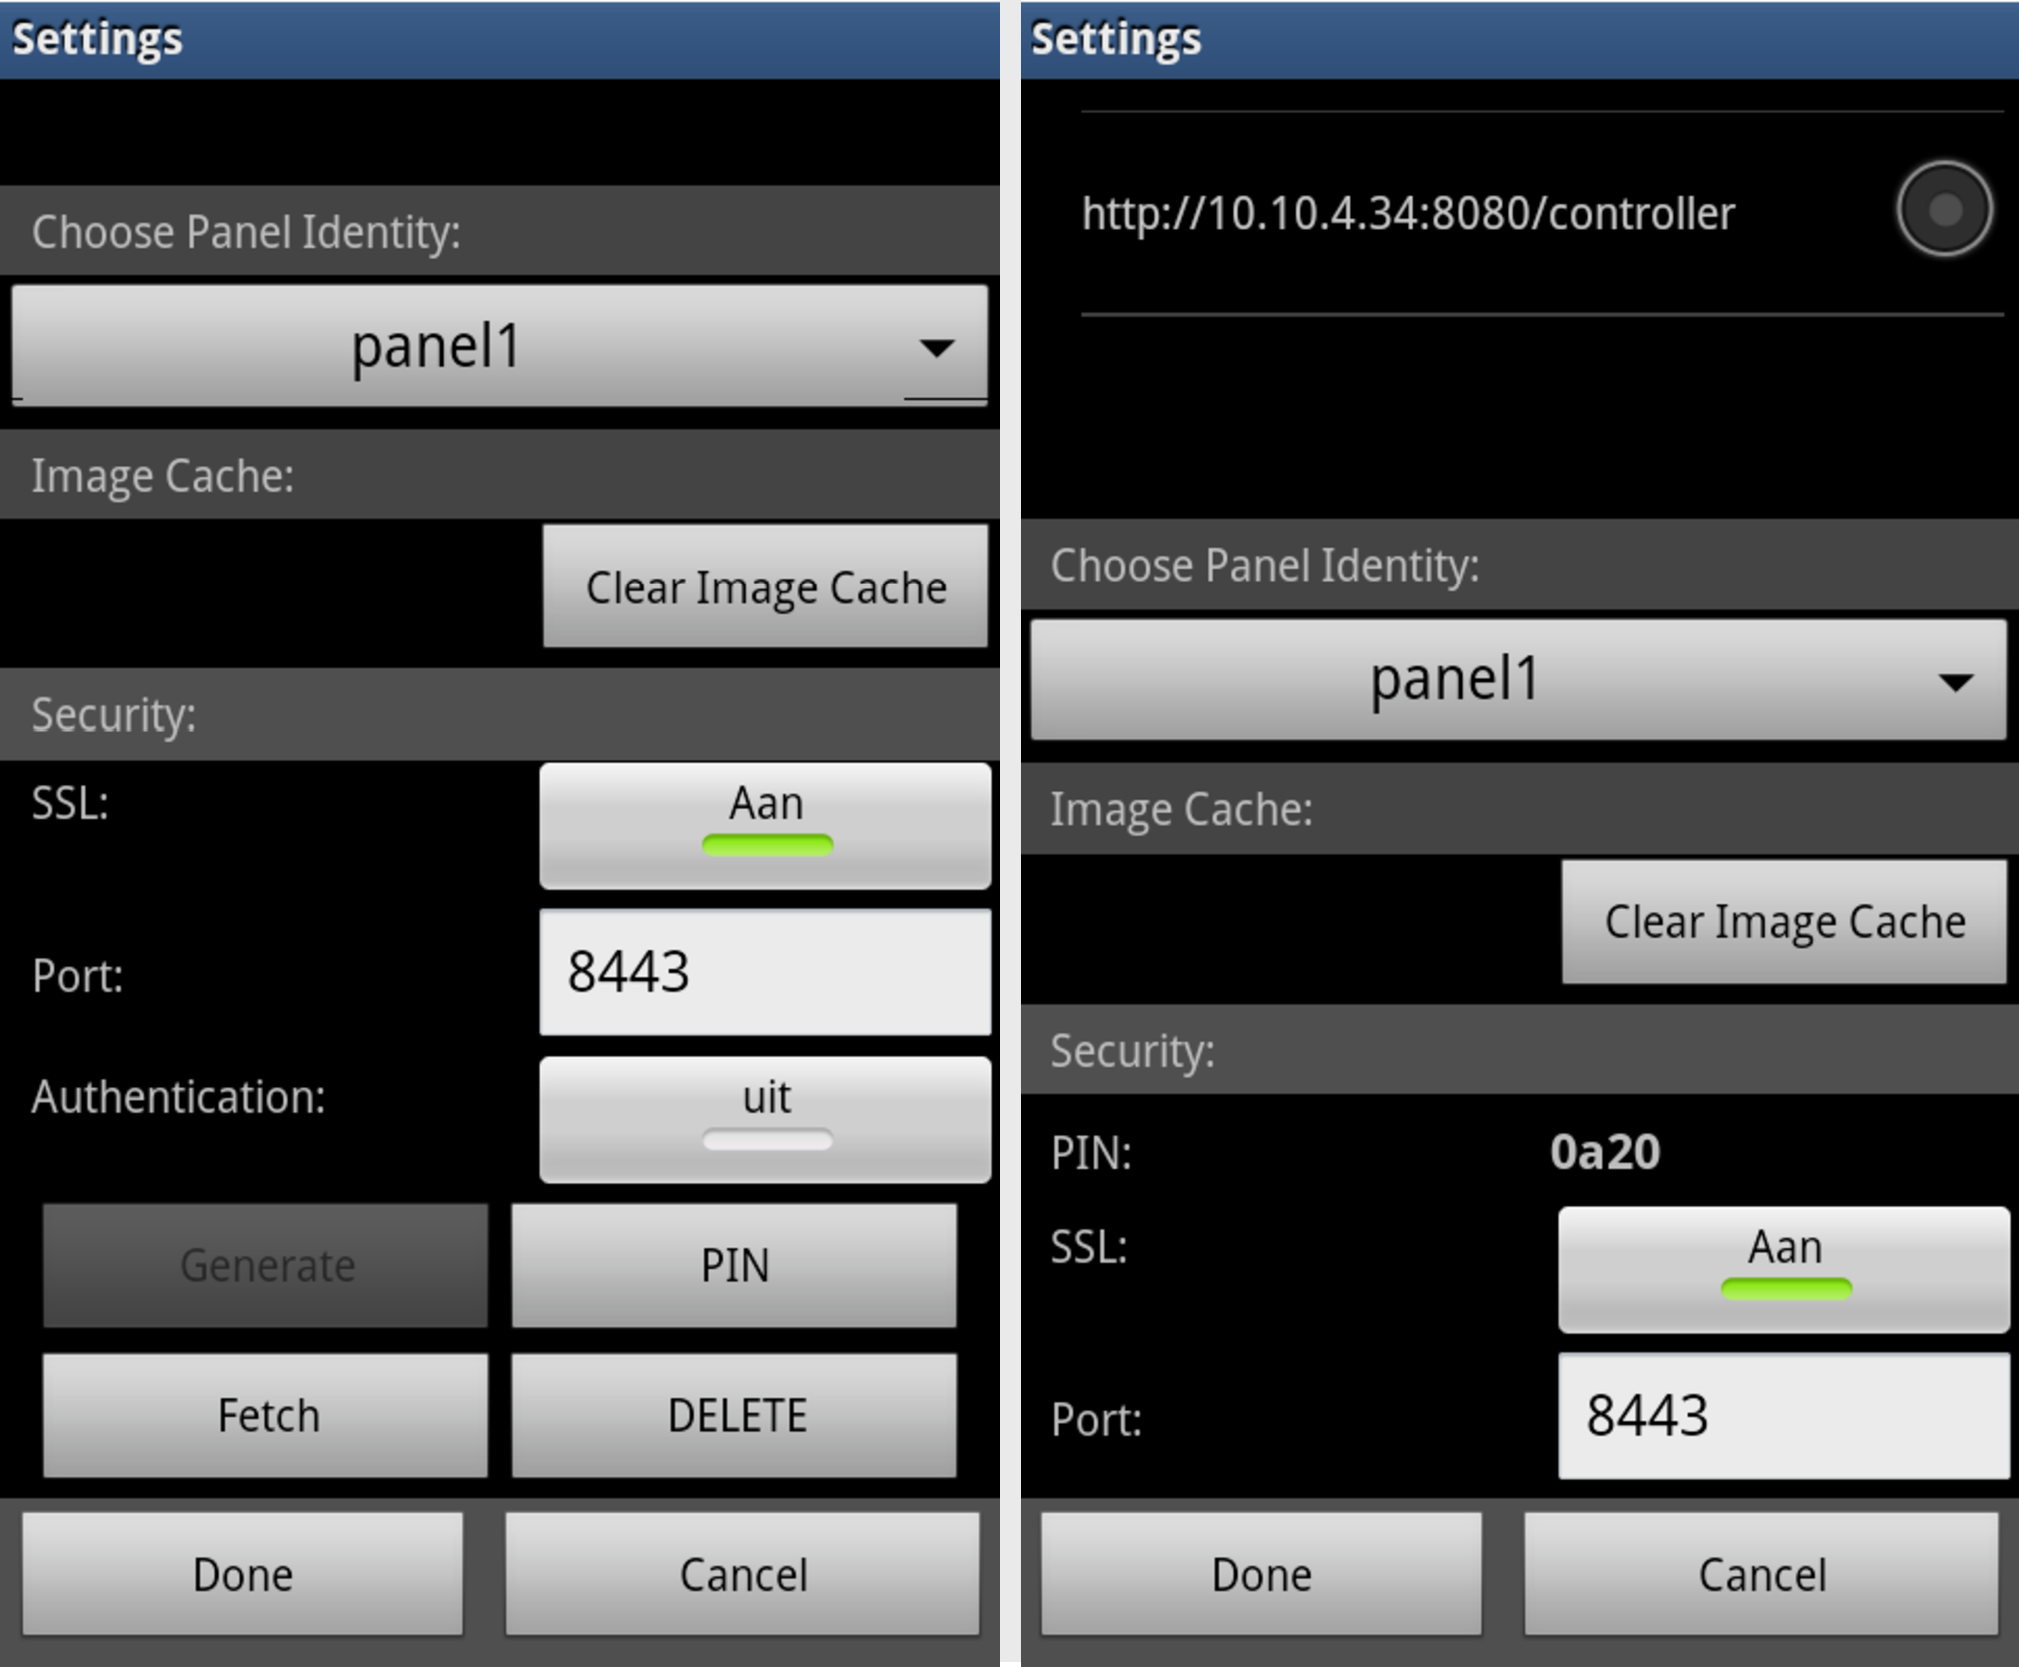
\includegraphics[height=0.4\textheight]{device-android.pdf}
   \end{center}
   \caption{Verschil tussen Android interfaces}
   \label{androidv2}
\end{figure}

In latere versies is de interface dermate geoptimaliseerd dat deze knoppen niet
meer nodig zijn. De vernieuwde interface, te zien in figuur \ref{androidv2}, heeft een
veld waar de PIN direct af te lezen is zonder pop-up. De knoppen zijn weggehaald
aangezien de acties nu automatisch gebeuren. Zo wordt er automatisch een
certificaat aangevraagd en opgehaald wanneer er verbinding wordt gemaakt. 

\subsection{Controller}
De OpenRemote Controller heeft een administrator panel om de gebruikers-/mobiele
apparaten te kunnen beheren. De beheerder kan inloggen met zijn/haar
inloggegevens van de Beehive server (Modeler account). Hierdoor zijn er geen
extra login gegevens nodig die onthouden zouden moeten worden. Er wordt communicatie
gelegd met de Beehive server, de login gegevens worden gestuurd naar de Beehive server
en vervolgens daar gecontroleerd. De Beehive server geeft vervolgens een 'OK'
of 'NOT ALLOWED' terug, waarna er met zekerheid te zeggen is dat de login gegevens
correct of incorrect zijn opgegeven.

Wanneer er geen rechtstreekse toegang is tot het internet op de 
OpenRemote Controller is het noodzakelijk om toch in te kunnen loggen met de
login gegevens van de Beehive server. Er is daarom gekozen bij de login module
om gebruik te maken van cache gegevens uit de database, om zodoende de administrator te
kunnen valideren.

Het is van groot belang dat deze gegevens veilig worden opgeslagen. Daarom is er
gekozen voor het opslaan van het wachtwoord in SHA512 (behoord tot de SHA-2
familie). Ook wordt bij de HTTP sessie id  wordt er gebruik gemaakt van het SHA512
hash algoritme. Voorheen was dit MD5 echter is dit relatief
eenvoudig te kraken via brute-force en/of rainbow table. Het voordeel van SHA512
is dat het gebruik maakt van 512 bits woord in tegenstelling tot 128
bits, waardoor het veel minder snel gekraakt kan worden.

Tenslotte is er een grafische interface gemaakt (te zien in figuur 12) om
apparaten goed en/of af te keuren vanuit de 'administrator panel'. Er bestaat
een PIN die vergeleken kan worden met de PIN die aanwezig is op het Android
apparaat. Indien de PIN van Android en de administrator panel overeenkomen, is
er met zekerheid te zeggen dat het hetzelfde apparaat betreft. Deze PIN is
gebaseerd op de publieke sleutel die ook aanwezig is in het client certificaat.

Naast 'User management' heeft het administrator panel ook een tab
'Configuration'. In deze tab is het mogelijk om bepaalde instellingen te
veranderen, zoals de authenticatie of de PIN check aan- of uit te zetten.  Het
administrator panel is beveiligd door een gebruikersnaam en wachtwoord die
overeen moeten komen met een bestaand OpenRemote Designer account. Op deze manier
is het administratie panel enkel toegankelijk voor de administrator.

Om te voorkomen dat het wachtwoord relatief eenvoudig te achterhalen is, wordt
er aangeraden om gebruik te maken van 'Pepper \& Salt' oftewel peper en zout. Met
deze termen wordt bedoeld dat het wachtwoord met een bepaalde random lijst
met karakters wordt uitgebreid (Salt), en een geheime constante (Pepper) wordt
toegevoegd. Er is gekozen om een systeem constante te gebruiken als zijnde
'Pepper' en een random lijst van karakters die gegeneerd wordt via het SHA-512
algoritme met een lengte van 32 bits die gebruikt wordt als 'Salt'. 

Uiteindelijk is er een grafische interface gemaakt om apparaten goed en/of af te
keuren vanuit het administrator panel. Er bestaat een PIN die vergeleken kan
worden met de PIN die aanwezig is op het Android apparaat. Indien de PIN van
Android en het administrator panel overeenkomen, is er met zekerheid te zeggen
dat het hetzelfde apparaat betreft. Deze PIN is gebaseerd op de publieke sleutel
die aanwezig is in het client certificaat. Naast 'User management' heeft het
administrator panel ook een tab, genaamd 'Configuration'. In deze tab is het
mogelijk om bepaalde instellingen te veranderen zoals de authenticiteit, of door
PIN check aan- of uit te zetten.  De administrator panel is beveiligd door een
gebruikersnaam en wachtwoord die overeen moeten komen met een bestaand
OpenRemote Designer account. Op deze manier is het administratie panel enkel
toegankelijk voor de administrator.

\begin{figure}[htpb]
   \begin{center}
     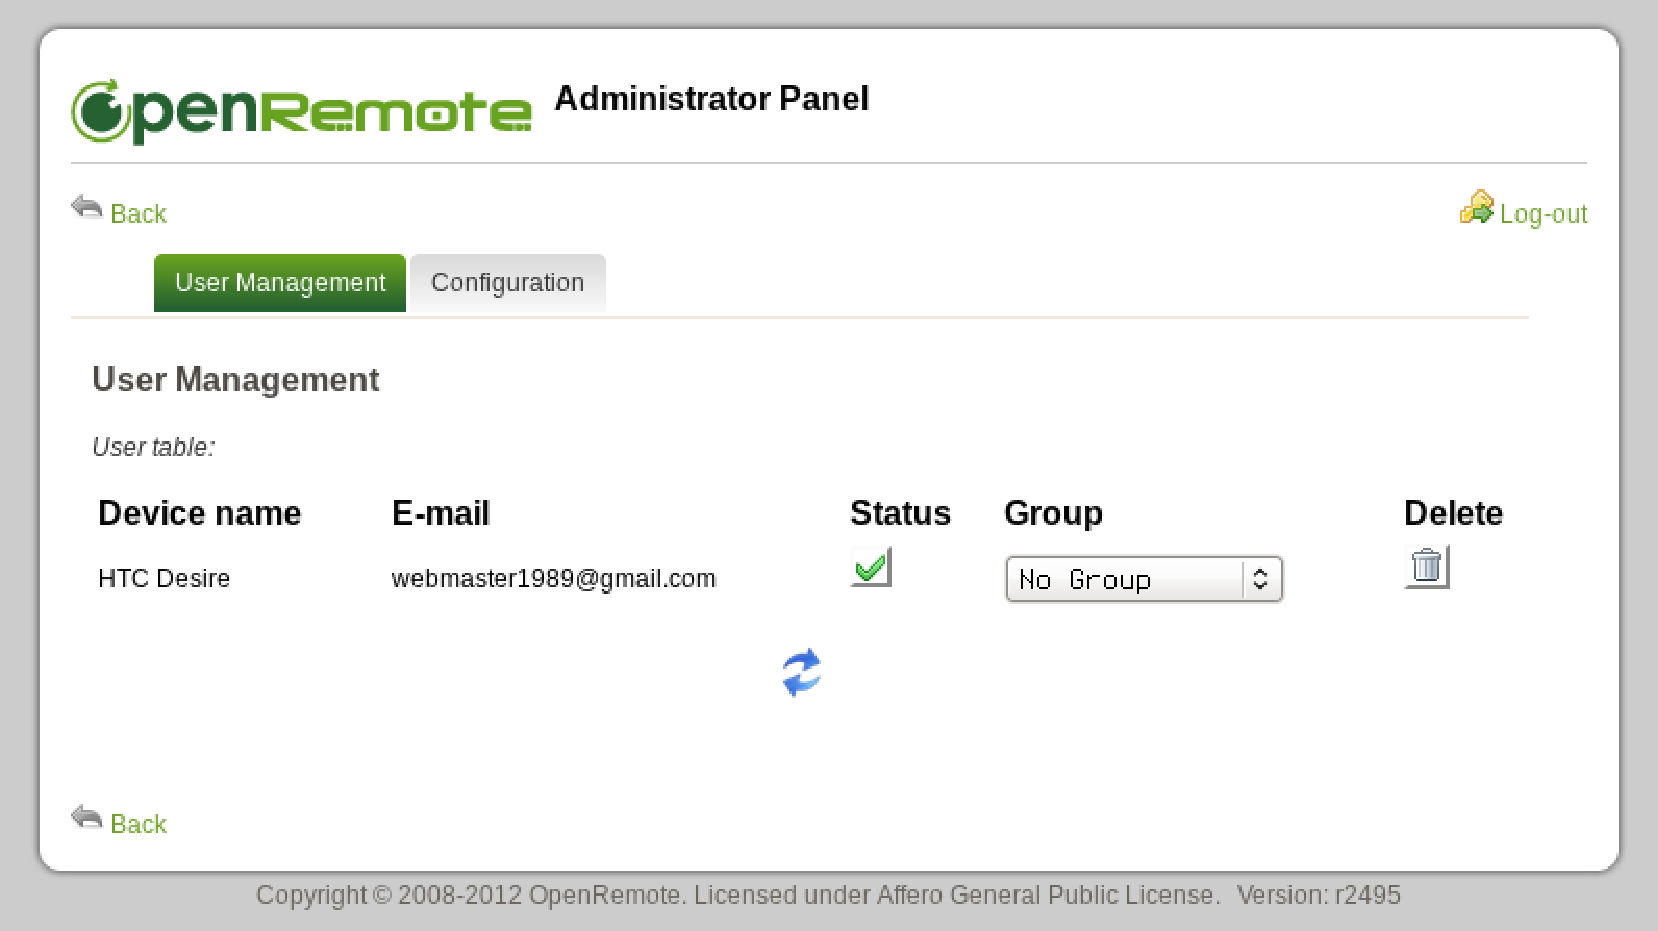
\includegraphics[width=0.6\textwidth]{userlist.pdf}
   \end{center}
   \label{userlist}
   \caption{Gebruikers management lijst}
\end{figure}

\subsection{Groepen}
Binnen het OpenRemote project bestond er veel vraag naar om apparaten in groepen aan
te kunnen geven. Aan deze vraag is in dit project gehoor gegeven. In de
OpenRemote Composer is er voor gezorgd dat aan de knoppen een groep toegewezen
kan worden. Deze groepen worden gekoppeld aan groepen in de beide xml bestanden
die ge\"exporteerd worden vanuit de server. Per knop kunnen meerdere groepen
gekoppeld worden.

Op de controller worden de groepen uit XML gehaald en in de database opgeslagen.
Vervolgens kan er in het admin panel een gebruiker aan een knop gekoppeld
worden zoals te zien in figuur \ref{usergroups}. De koppeling tussen gebruiker
en groep wordt opgeslagen in de database op de controller. 

Als er vervolgens een commando wordt gestuurd naar de controller, wordt de
gebruiker in de database opgezocht. Vervolgens wordt er gekeken welke groep aan
de gebruiker gekoppeld is. Ook wordt er gekeken welke groepen er aan het element
zitten waar een actie op wordt uitgevoerd. Als er een groep overeenkomt, wordt
de actie uitgevoerd. Zo niet, dan wordt er een errorcode teruggegeven.

In de android applicatie wordt er bij het tekenen van de knoppen gekeken welke
groep er aan deze knop gekoppeld zit en tot welke groep de gebruiker behoort.
Als de gebruiker geen toegang heeft tot de knop, wordt deze disabled en kan deze
dus niet ingedrukt worden.

\begin{figure}[htpb]
   \begin{center}
     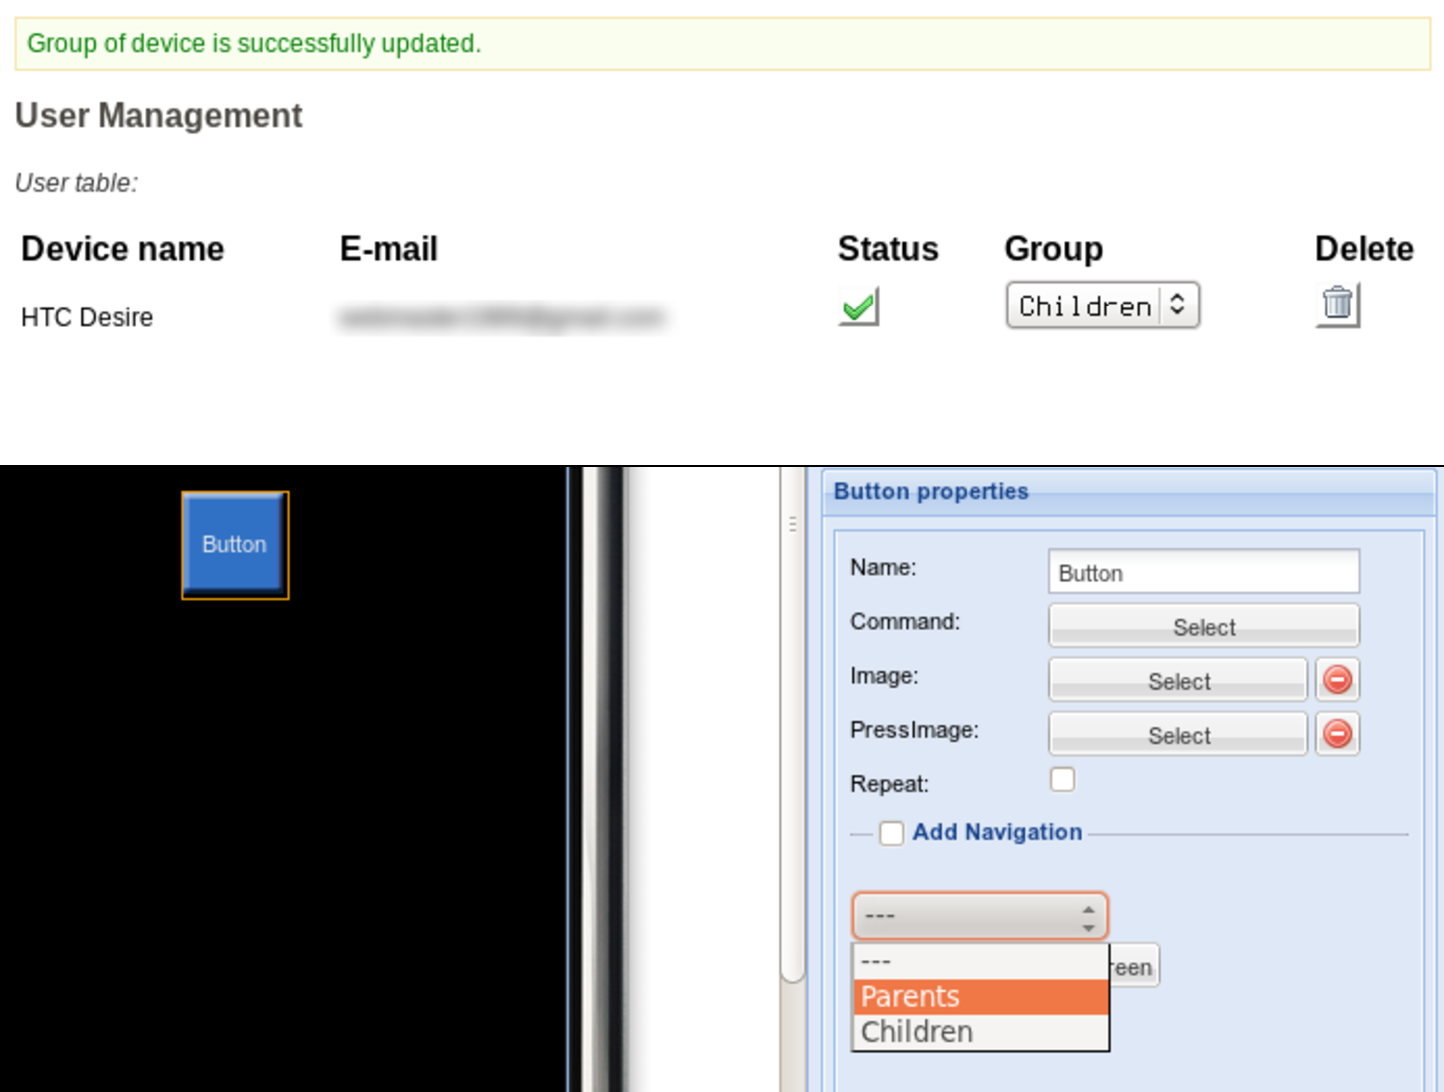
\includegraphics[width=0.6\textwidth]{usergroups.pdf}
   \end{center}
   \caption{Gebruikers koppelen aan groepen}
   \label{usergroups}
\end{figure}

\newpage
\section{Resultaten}

Tijdens de afstudeerperiode zijn er resultaten geboekt die vermeld zijn in dit
hoofdstuk. Hier wordt per iteratie uitgelegd welke resultaten behaald
zijn en aan welke eisen deze moesten voldoen.

\subsection{Iteratie 1: Onderzoek}
Voor de eerste iteratie is onderzoek gedaan in het werkveld van de afstudeerstage.
Er is onderzoek gedaan naar vier delen: Domotica protocollen, domotica hardware,
PlugTops en OpenRemote met alternatieven. 

\begin{table}[htpb]
  \caption{Eisen iteratie 1: Onderzoek}
  \begin{center}
    \begin{tabular}{|| l ||}\hline
        Eis                                                  \\\hline\hline
        Uitzoeken protocollen en onderzoeksdocument opzetten \\\hline
        Uitzoeken PlugTop en onderzoeksdocument opzetten     \\\hline
        Uitzoeken Hardware en onderzoeksdocument opzetten    \\\hline
        Uitzoeken OpenRemote en onderzoeksdocument opzetten  \\\hline
    \end{tabular}
  \end{center}
\end{table}

Het doel van deze iteratie is het scheppen van opheldering over de mogelijke
keuzes. Er is onderzocht welke domotica protocollen er bestaan en welke het
meest geschikt zijn voor toepassing in het project. Uit dit onderzoek is
gebleken dat X10 het meest gebruikte, voordeligste en veelzijdigste protocol op de markt
is. Ook is Z-Wave een mooi protocol aangezien het draadloos werkt. Echter
Z-Wave is duurder en deze wordt minder goed ondersteund. Dat betekent dat het voor dit
project minder geschikt is, en daarom is de keuze op X10 gevallen.  

Het PlugTop onderzoek heeft aangetoond dat de binnen TASS gebruikte
DreamPlug de meest geschikte PlugTop voor dit project is. De DreamPlug
beschikt over een groot aantal aansluitingen en is gunstig geprijsd. 

In het onderzoek naar OpenRemote is gekeken naar de mogelijkheden van het
OpenRemote project in vergelijking met andere software pakketten. Hieruit is 
gebleken dat OpenRemote beschikt over de meeste mogelijkheden en het meest
actief wordt bijgehouden. Wel is de beveiliging van OpenRemote niet heel
goed geregeld. In bijlage 6 is het onderzoek te vinden.

\subsection{Iteratie 2: Testopstelling}
\begin{table}[htpb]
  \caption{Eisen iteratie 2: Testopstelling}
  \begin{center}
    \begin{tabular}{|| l ||}\hline
        Eis                                                              \\\hline\hline
        Als gebruiker wil ik een Android applicatie om een lamp aan en   \\ 
        uit te zetten                                                    \\\hline
        Als klant wil ik weten wat voor autorisatie en authenticatie    \\
        methoden er bestaan.                                             \\\hline
    \end{tabular}
  \end{center}
\end{table}

Tijdens de tweede iteratie is er gewerkt aan het opzetten van een
testopstelling met OpenRemote, de DreamPlug en de X10 hardware. Ook is er
onderzoek gedaan naar verschillende beveilingsmethodieken en oplossingen.

\begin{wrapfigure}{r}{0.4\textwidth}
  \begin{center}
    
\includegraphics[width=0.20\textwidth]{android.pdf}
  \end{center}
  \caption{Android}
\end{wrapfigure}

Met de testopstelling is het mogelijk om een lamp
aan te sturen met de OpenRemote controller, welke draait op de
DreamPlug. Met de OpenRemote app is het mogelijk om met behulp van deze
opstelling een lamp aan te zetten via een X10 stopcontactmodule.

Het onderzoek naar beveiliging concludeert dat de beste methode om
OpenRemote te beveiligen het gebruik van SSL certificaten is. Deze
certificaten kunnen door zowel de server als de client gebruikt worden om
zich te authenticeren. Zie bijlage 4 voor meer informatie.

\subsection{Iteratie 3: SSL Proof-of-Concept}
De derde iteratie heeft in het teken gestaan van de Proof-of-Concept die laat zien
dat het mogelijk is om met Android te verbinden naar een TomCat server en
te authenticeren door middel van SSL Client Certificaten.

\begin{table}[htpb]
  \caption{Eisen iteratie 3: SSL Proof-of-Concept}
  \begin{center}
    \begin{tabular}{|| l ||}\hline
        Eis                                                              \\\hline\hline
        Als beheerder wil ik zien welke apparaten er zijn aangemeld      \\\hline
        Als systeem wil ik onderscheid zien tussen verschillende devices \\\hline
        Als gebruiker wil ik zien dat mijn telefoon uniek                \\ 
        identificeerbaar is                                              \\\hline
    \end{tabular}                                                         
  \end{center}                                                            
\end{table}                                                               

Voor de Proof-of-Concept zijn er een aantal eisen. Als eerste moet de client
een aanvraag kunnen doen bij de server voor een certificaat. Deze aanvraag
moet in een lijstje te zien zijn waarna er een certificaat terug wordt
gestuurd naar de client. Dit certificaat wordt gegenereerd op de server,
ge\"encodeerd met Base64 en overgestuurd naar de client.

De beheerder kan op de server een lijst met aanvragen zien evenals een
lijst met gebruikers die daadwerkelijk een certificaat hebben. Er is in deze
sprint nog niet gewerkt aan het dynamisch genereren van certificaten voor
gebruikers. Dit wordt in deze versie nog automatisch gedaan, in de volgende
iteraties zal deze functionaliteit toegevoegd worden.

Er is ook voor gezorgd dat de gebruikers uniek identificeerbaar zijn. De server
en client moeten kunnen zien dat de client uniek identificeerbaar is. Er wordt
gebruik gemaakt van het 'serial' attribuut wat in elk certificaat aanwezig is.
Dit attribuut is een oplopende integer.

\subsection{Iteratie 4: SSL in OpenRemote}
In de daaropvolgende iteratie is er gewerkt aan het implementeren van de
Proof-of-Concept in het OpenRemote project.

Er zijn een aantal onderdelen verbeterd om ze te kunnen implementeren in het
OpenRemote project. Het administrator panel
is een onderdeel hiervan. Deze interface is verbeterd, hij is
ontworpen (zie figuur \ref{adminv1}) en er zijn acties aan gekoppeld 
waarmee de client goedgekeurd kan worden.

\begin{table}[htpb]
  \caption{Eisen iteratie 4: SSL in OpenRemote}
  \begin{center}
    \begin{tabular}{|| l ||}\hline
        Eis                                                              \\\hline\hline
        Als beheerder wil ik sommige gebruikers toestemming geven in een \\ 
        webinterface                                                     \\\hline
        Als gebruiker wil ik met de android app van OpenRemote client    \\ 
        certificaten gebruiken om te verbinden met de server             \\\hline
        Als gebruiker wil ik met de android app van OpenRemote een client\\
        certificaat op kunnen halen van de server                        \\\hline
        Als beheerder wil ik een lijst zien met gebruikers in een        \\ 
        webpagina op de openremote controller                            \\\hline
        Als beheerder wil ik clients toestemming kunnen geven door middel\\ 
        van een PIN uit te wisselen en te controleren in de web interface\\\hline
    \end{tabular}
  \end{center}
\end{table}

Van deze clients kan informatie getoond worden, namelijk het emailadres,
de naam van de telefoon en een PIN. Deze PIN wordt gegenereerd door een
hash van de publieke sleutel te maken en daarvan de laatste 4 karakters te
laten zien.

\begin{figure}[h!]
  \centering
    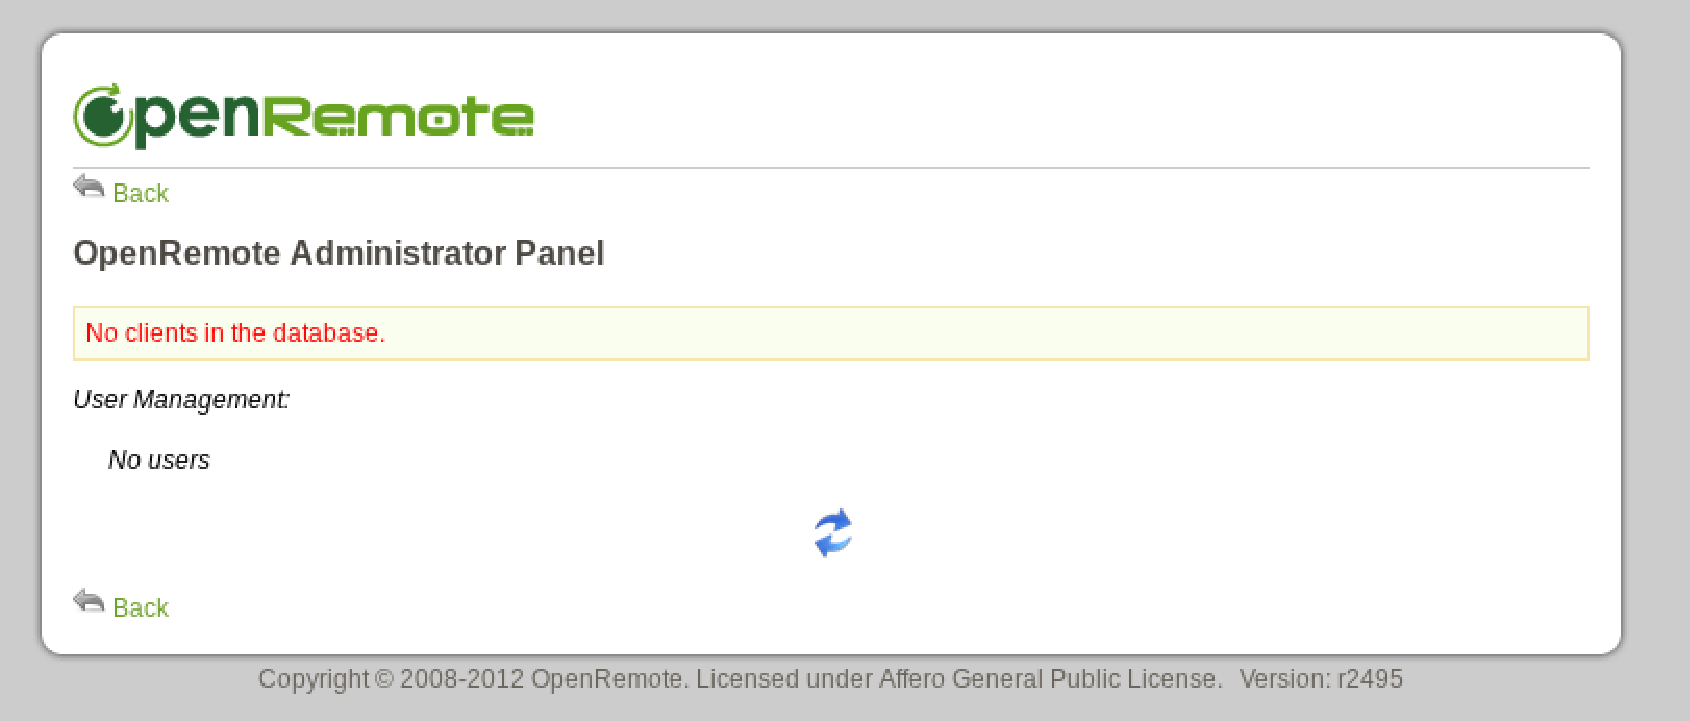
\includegraphics[height=150pt,keepaspectratio]{adminv1.pdf}
  \caption{Ontwerp administrator panel}
  \label{adminv1}
\end{figure}

De app stuurt sinds deze iteratie een CSR (Certificate Signing Request) naar de server. De server
gebruikt deze CSR om een certificaat te maken. Op deze manier wordt de private
sleutel van de client nooit overgestuurd en kan deze ook niet onderschept
worden door kwaadwillenden.

\subsection{Iteratie 5: Platformonafhankelijkheid}
\begin{table}[htpb]
  \caption{Eisen iteratie 5: Platformonafhankelijkheid}
  \begin{center}
    \begin{tabular}{|| l ||}\hline
        Eis                                                              \\\hline\hline
        Als beheerder wil ik in kunnen loggen met de gegevens van        \\
        http://composer.openremote.org                                   \\\hline
        Als beheerder wil ik de toegang van clients kunnen intrekken van \\ 
        het systeem om de toegang te ontzeggen                           \\\hline
        Als beheerder wil ik de OpenRemote Controller op alle            \\ 
        verschillende platformen kunnen installeren                      \\\hline
        Als gebruiker wil ik de interface zo simpel mogelijk maken       \\\hline
    \end{tabular}
  \end{center}
\end{table}

In de vijfde iteratie is er voor gezorgd dat alle platformen ondersteund worden.
OpenRemote is een cross platform applicatie. De Controller draait op TomCat
welke in Java geschreven is. Dit betekent dat het draait op elk platform waar
Java draait. Echter hebben de wijzigingen, die in de vorige iteratie zijn
doorgevoerd, er voor gezorgd dat het noodzakelijk is toegang te hebben tot
het 'openssl' commando. In deze iteratie is gewerkt aan het vervangen van het
'openssl' commando door de Bouncy Castle library, wat ervoor zorgt dat de
cryptografische acties gebeuren door middel van Java, in plaats van een aanroep
naar openssl. 

In bijlage 2 is te zien wat er gebeurt als er een
aanvraag binnenkomt bij de Controller. De client doet in het begin een aanvraag
voor toegang. Hiermee stuurt hij een CSR bestand op waar al zijn gegevens in staan,
welke de Controller gebruikt om een certificaat te maken. 

Als er een aanvraag binnenkomt, voegt de Controller de nieuwe client toe aan de
database. De gegevens in de database worden uit de CSR gehaald. Vervolgens is de
client te zien in de beheerdersinterface. Hij is nog niet
goedgekeurd en heeft dus ook geen toegang tot het systeem.

Wanneer de beheerder de client goedgekeurd heeft, en desgewenst de PIN ingevoerd
heeft, wordt het certificaat gegenereert. Als eerste
wordt de private key van de CA opgehaald. Elk certificaat dat gemaakt wordt,
wordt ondertekend door de CA. Deze CA wordt ook geimporteerd in de OpenRemote
Controller en op die manier weet OpenRemote dat hij de clients kan vertrouwen.

Daarna wordt de private key samen met de CSR gebruikt om een certificaat te
cree\"eren. Tevens moet er een serienummer meegegeven worden. Dit serienummer is een
uniek oplopend nummer waarmee de certificaten te identificeren zijn. Het
certificaat dat gemaakt is wordt in een keystore
opgeslagen, klaar om opgehaald te worden door de mobiele applicatie. Tevens wordt de
status van de client in de database aangepast.

Nu kan de gebruiker met de applicatie een certificaat ophalen en met dit
certificaat een veilige verbinding opzetten. Tevens kan TomCat het certificaat
gebruiken om de gebruiker te identificeren. In de database staat de 'dname'
welke ook in het certificaat staat. Op het moment dat een client een verbinding
maakt met TomCat, controleert TomCat de dname en kijkt in de database of deze
gebruiker toegang heeft tot het systeem. Mocht dat niet het geval zijn, dan zal hij
de gebruiker geen toegang tot het systeem geven.
Zie bijlage 2.

Tevens is er een configuratiescherm gemaakt. In dit scherm kunnen een aantal dingen worden
ingesteld, zoals onder andere het pad waar de CA opgeslagen wordt en of de PIN
verplicht gecontroleerd moet worden.

\begin{figure}[h!]
  \centering
    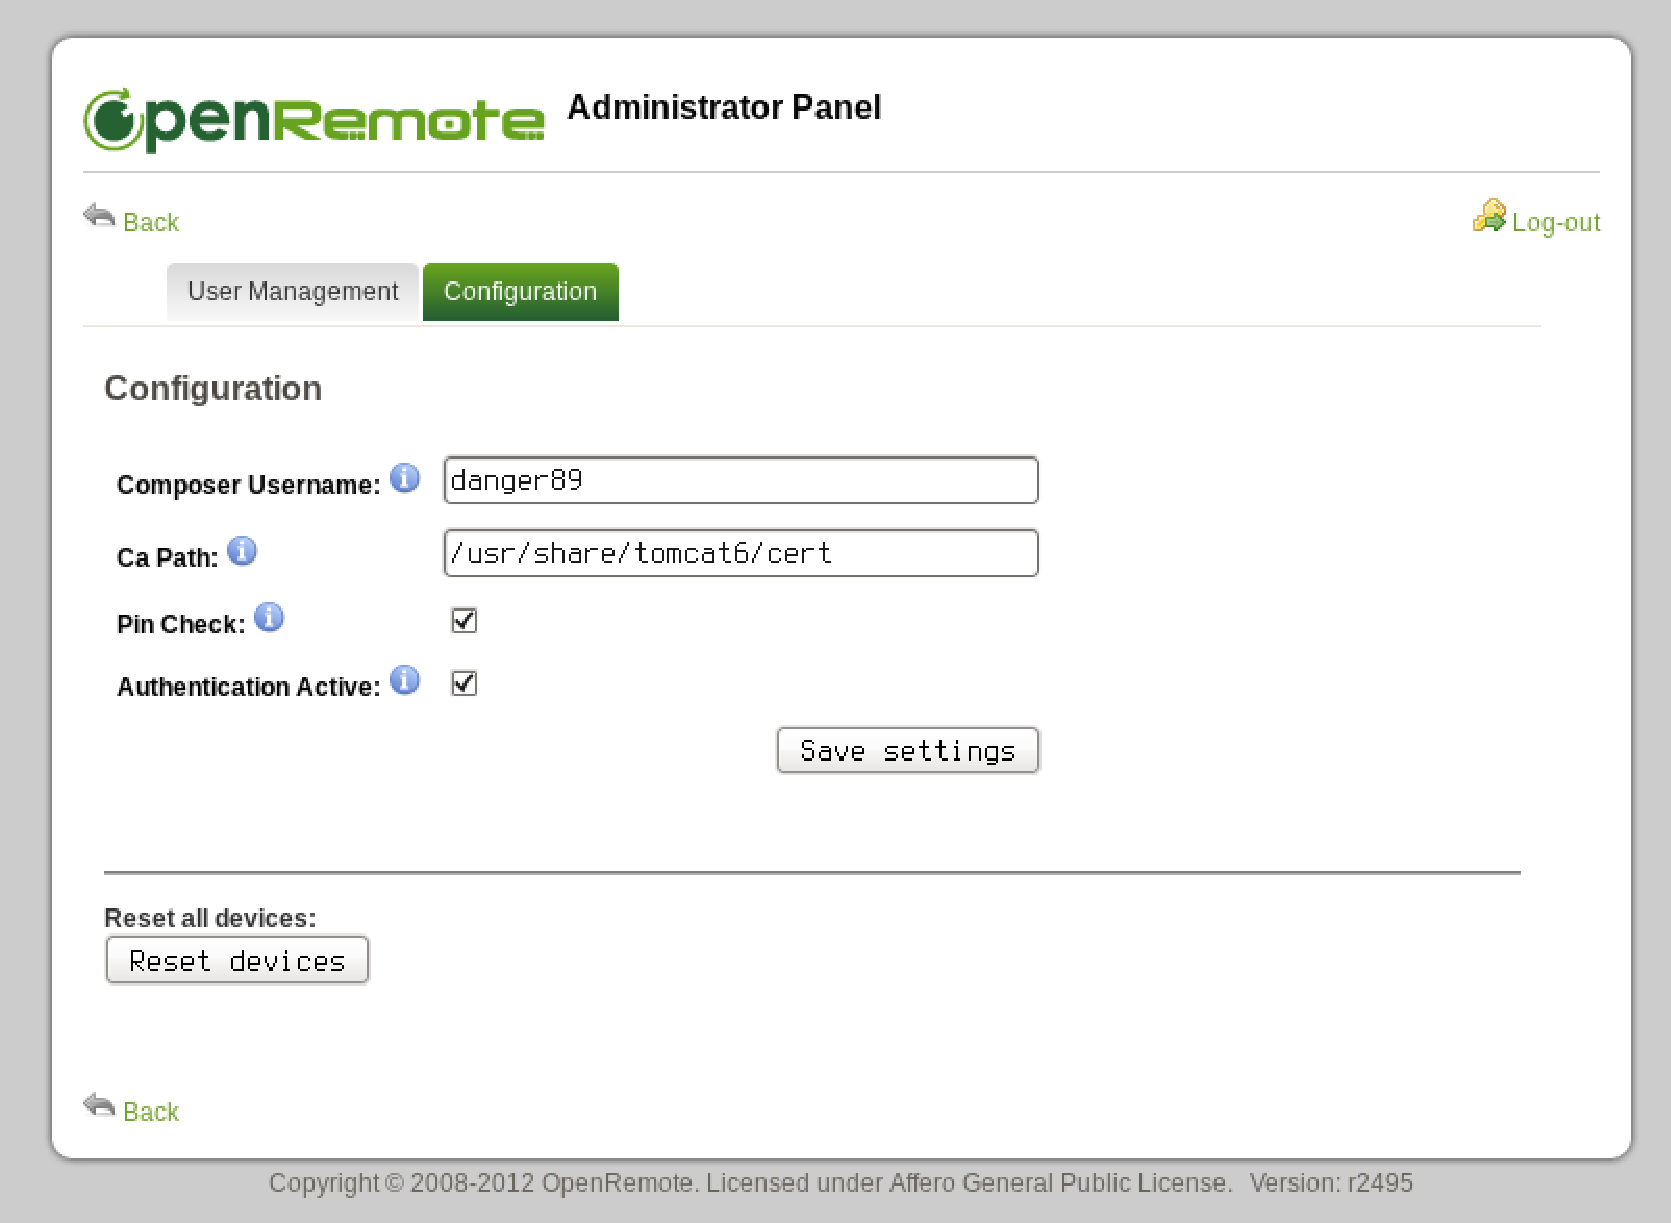
\includegraphics[width=0.7\textwidth,keepaspectratio]{adminv2config.pdf}
  \label{adminv2config}
  \caption{Het configuratiescherm}
\end{figure}

Dit configuratiescherm en het user managementscherm, samen het administrator
panel, zijn beide beveiligd met
een gebruikersnaam en wachtwoordcombinatie. Deze combinatie is dezelfde als
waarmee ingelogd wordt op \url{http://composer.openremote.org/demo/}. 
Deze worden online gecontroleerd als er ingelogd wordt. Mocht er geen
internetverbinding zijn, dan wordt de cache uit de database gebruikt.

\subsection{Iteratie 6: Oplevering naar OpenRemote}
\begin{table}[htpb]
  \caption{Eisen iteratie 6: Oplevering naar OpenRemote}
  \begin{center}
    \begin{tabular}{|| l ||}\hline
        Eis                                                              \\\hline\hline
        Als beheerder wil ik authenticatie en autorisatie uit kunnen    \\
        schakelen om terug te vallen op de standaard onbeveiligde        \\ 
        verbinding                                                       \\\hline
        Als gebruiker wil ik alleen via SSL port \& client certificaten  \\ 
        bij de OpenRemote Controller kunnen komen                        \\\hline
        Als ontwikkelaar wil ik documentatie hebben over de implementatie\\ 
        van het authenticatie systeem                                    \\\hline
        Als ontwikkelaar wil ik een patch hebben van de toevoegingen ten \\
        opzichte van een OpenRemote release                              \\\hline
    \end{tabular}
  \end{center}
\end{table}

In de zesde iteratie van dit project is er gewerkt aan het opleveren van een
stabiele release voor de ontwikkelaars van OpenRemote. Zoals eerder vermeld is
er in dit project gewerkt aan het uitbreiden van een bestaand open source
project, namelijk OpenRemote. 

Er is voor gezorgd dat voor het verbinden met SSL client certificaten verplicht
gesteld kunnen worden. Dit betekent dat vanaf deze iteratie het alleen mogelijk is
om te verbinden met de Controller met behulp van een bekend SSL Client
Certificaat. Er wordt, als er verbinding is, gecontroleerd of het client certificaat bekend
is bij de Controller. Zo ja, dan is er toegang, anders niet.

Ook is ervoor gezorgd dat de uitbreidingen op OpenRemote uit te zetten
zijn. Er is een checkbox bijgekomen in het configuratie paneel welke, als
deze uitgevinkt wordt, er voor zorgt dat TomCat niet meer controleert op client
certificaten. 

Tevens is er ook contact opgenomen met OpenRemote om de vorderingen te tonen.
Dit is gedaan via een bericht op het forum van OpenRemote, welke te vinden is via
de volgende link 
\url{http://openremote.org/pages/viewpage.action?pageId=19439381&focusedCommentId=19440285#comment-19440285}. 
In de forum post is kort uitgelegd wat de veranderingen zijn waar aan gewerkt is en hoe dit getest is. 
 
\subsection{Iteratie 7: Groepen}

In deze iteratie is er gewerkt aan het implementeren van groepen in OpenRemote.
Deze functie houdt in dat men een groep toe kan wijzen aan een knop in de layout
designer, en een telefoon/tablet aan een groep toe kan wijzen. Op het moment dat er
een device en een knop in dezelfde groep zitten, zal de actie die aan de knop
hangt doorgevoerd worden.

\begin{table}[htpb]
  \caption{Eisen iteratie 7: Groepen}
  \begin{center}
    \begin{tabular}{|| l ||}\hline
        Eis                                                              \\\hline\hline
        Als beheerder kan ik groepen aanmaken om gebruikers in te delen  \\\hline
        Als beheerder kan ik gebruikers toewijzen aan groepen om         \\ 
        gebruikers rechten te geven                                      \\\hline
        Als beheerder kan ik knoppen toewijzen aan groepen om groepen    \\ 
        rechten te geven                                                 \\\hline
    \end{tabular}
  \end{center}
\end{table}

De modeler is uitgebreid met de mogelijkheid om groepen aan te maken, en
vervolgens deze groepen toe te kunnen wijzen aan 'besturingselementen'. Er kan
nu een groep toegewezen worden aan een knop, een switch en een slider. In de XML,
die vervolgens gegenereerd wordt, zijn ook de groepen toegevoegd. 

In de controller kan een gebruiker toegewezen worden aan een groep. Deze groepen
zijn hetzelfde als de groepen die worden aangemaakt in modeler en worden
meegestuurd in de XML. Standaard heeft een gebruiker geen groep, en dus geen
rechten, en in het administrator panel kan een groep toegewezen worden.

Mocht er toch op een knop gedrukt worden op de android applicatie, dan wordt er een
melding getoond met daarin het bericht dat de gebruiker niet in de correcte
groep zit. 

\subsection{Iteratie 8: Meer groepen}

\begin{table}[htpb]
  \caption{Eisen iteratie 8: Meer groepen}
  \begin{center}
    \begin{tabular}{|| l ||}\hline
        Eis                                                              \\\hline\hline
        Als beheerder kan ik knoppen aan meerdere groepen toewijzen om zo\\
        meer gebruikers er rechten toe te geven                          \\\hline
        Als gebruiker wil ik de knoppen die ik niet aan kan sturen niet  \\ 
        kunnen bedienen                                                  \\\hline
    \end{tabular}
  \end{center}
\end{table}

In deze sprint was het belangrijk om de groepen uit te breiden. In de modeler was
het nog niet mogelijk om meerdere groepen te selecteren voor \'e\'en knop.
Daarom is er in deze iteratie een nieuw scherm ontworpen en ge\"implementeerd
om gebruiksvriendelijk meerdere groepen te kunnen selecteren.

\begin{figure}[h!]
  \centering
    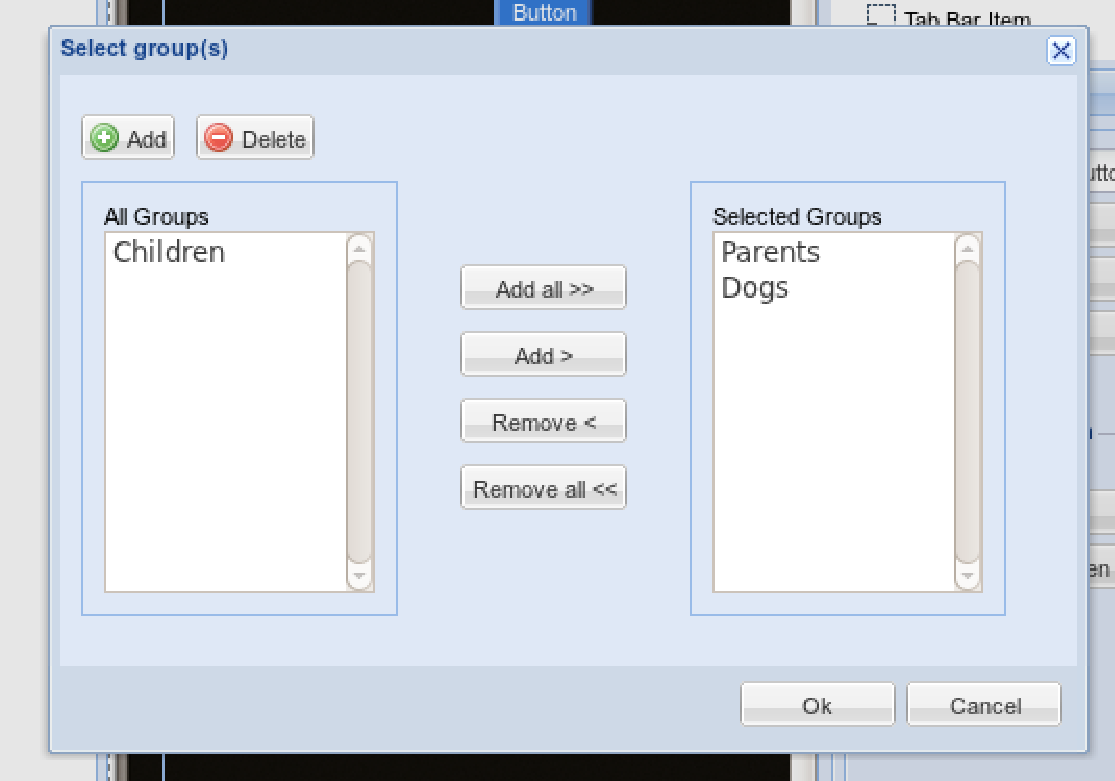
\includegraphics[width=0.6\textwidth,keepaspectratio]{groupselect.pdf}
  \caption{Het scherm waar groepen geselecteerd kunnen worden}
  \label{groupselect}
\end{figure}

Ook is er in deze iteratie voor gezorgd dat de knoppen die niet aangestuurd
mogen worden, op Android ook daadwerkelijk uitgeschakeld worden. Dit betekent dat
de knoppen donkergrijs worden gekleurd en niet meer in te drukken zijn.

%%
%Screenshot android applicatie met de knopen die uitgeschakeld zijn
%%

\subsection{Eindresultaat}
Aan het eind van de stage heeft de OpenRemote Modeler de mogelijkheid om groepen
toe te voegen. Deze groepen kunnen tevens ook verwijderd worden. Dezelfde
groepen kunnen aan knoppen, sliders en switches gekoppeld worden. Deze koppeling
gaat via een popup, welke te zien is in figuur \ref{groupselect}. Deze groepen
worden opgeslagen in xml en zo overgestuurd naar de controller.

De controller heeft een adminstrator panel gekregen. Deze heeft verschillende
opties, de belangrijkste is de gebruikerslijst (te zien in figuur
\ref{userlist}). In deze lijst staan de gebruikers die een aanvraag hebben
gedaan. In de configuratie tab kunnen de instellingen van de controller
aangepast worden, zoals te zien in figuur \ref{configv2}. 

\begin{figure}[h!]
  \centering
    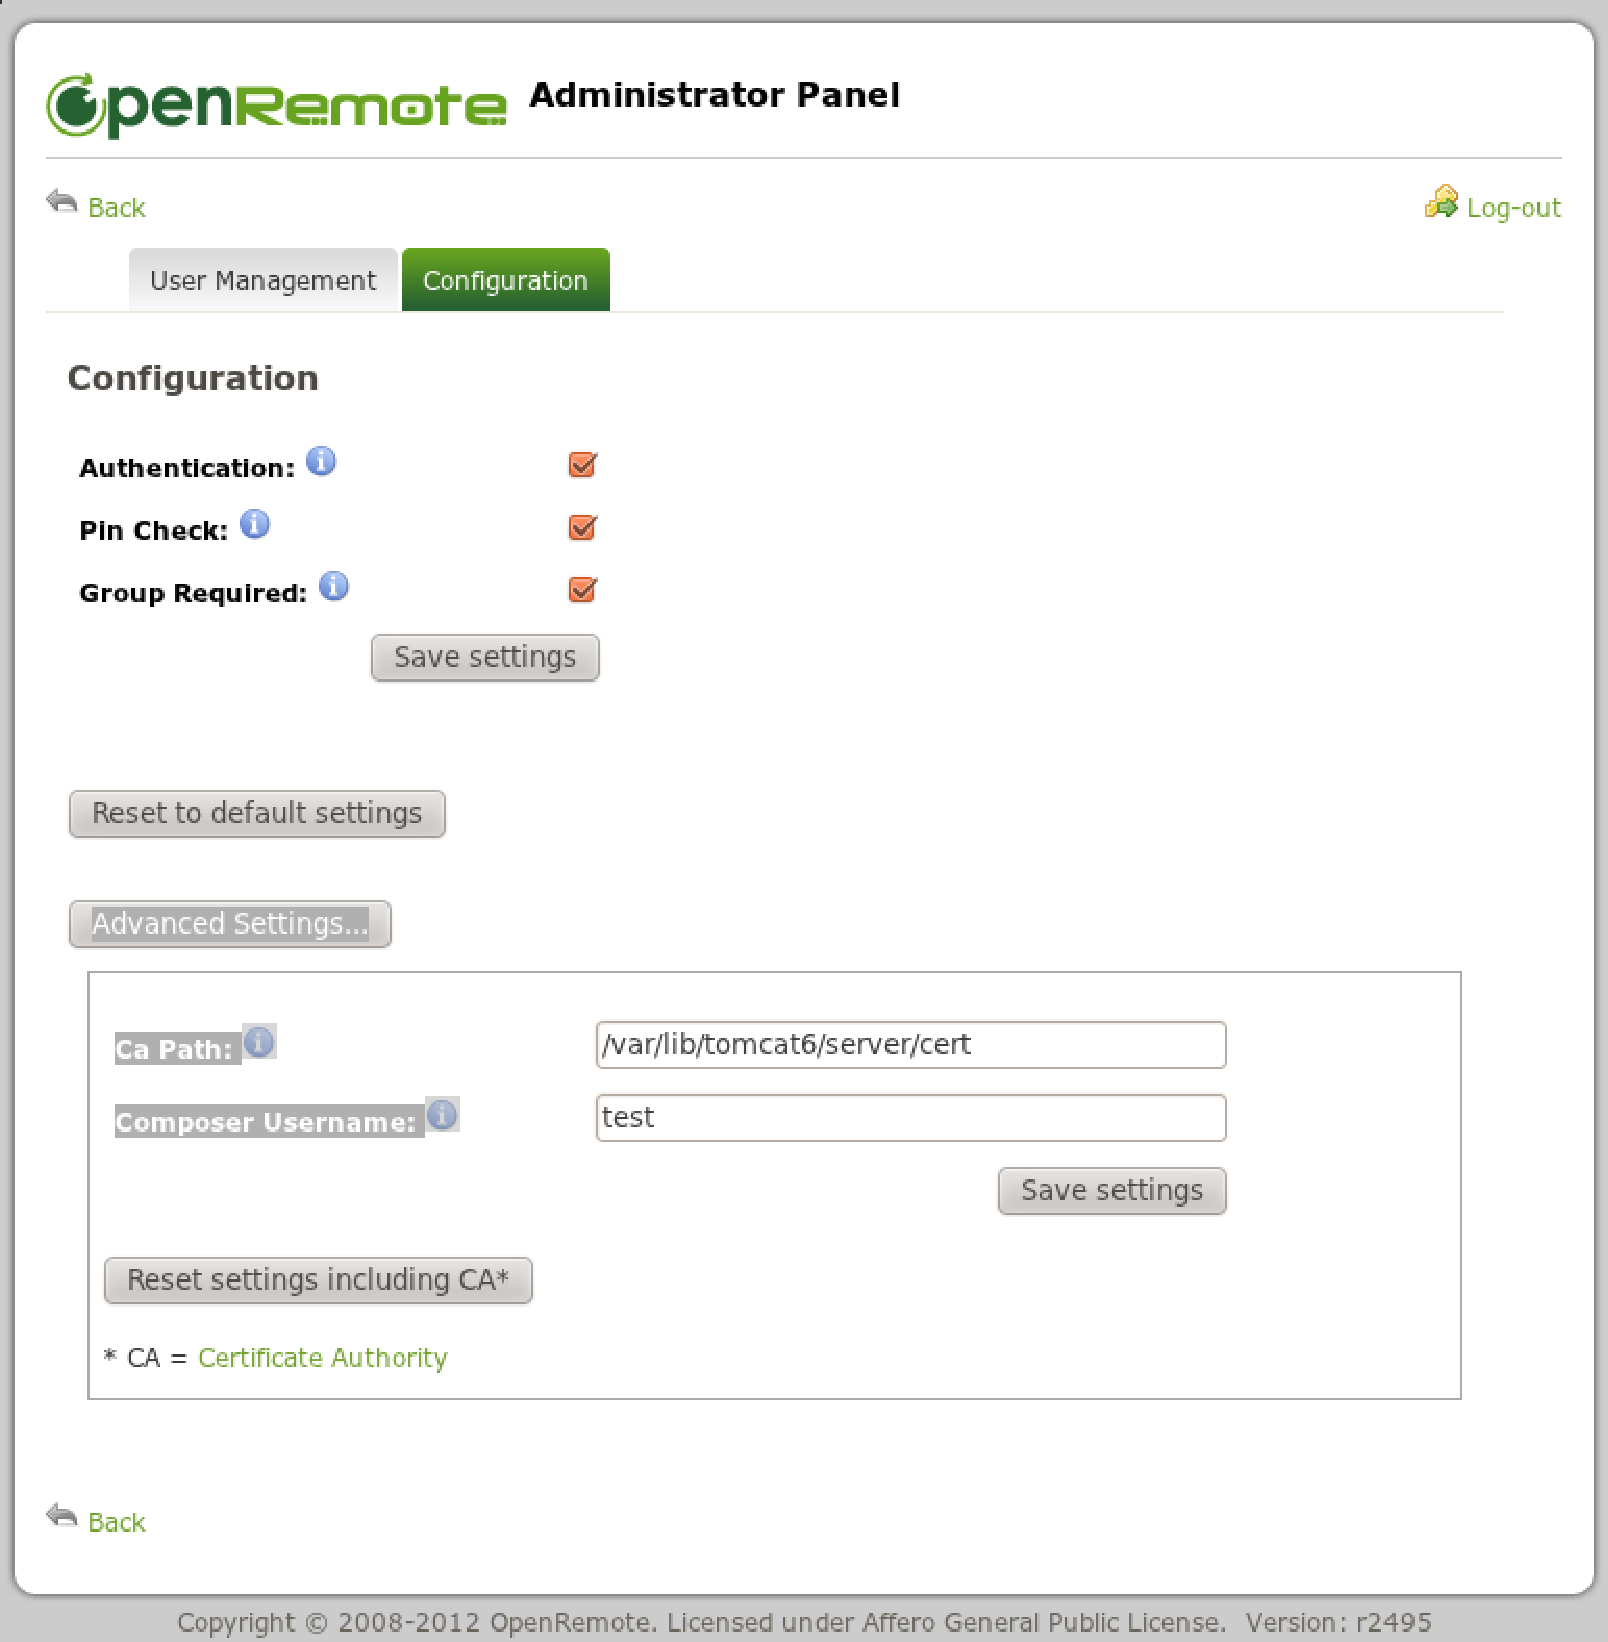
\includegraphics[width=0.6\textwidth,keepaspectratio]{configv2.pdf}
  \caption{Vernieuwde configuratie panel}
  \label{configv2}
\end{figure}

De controller vereist, als dat ingesteld is, een client certificaat van de
gebruiker. Deze certificaten kunnen, als de client ze nog niet heeft,
aangevraagd worden bij de controller. De controller gebruikt dan zijn CA om een
certificaat te maken voor de desbetreffende clients. 

Ook controleert de controller bij een aanvraag of de client in de juiste groep
zit. Zo niet, dan wordt de aanvraag niet verwerkt en wordt er dus geen domotica
apparatuur aangesproken. 

De android client kan, wanneer er een verbinding wordt gemaakt met de server,
een certificaat aanvragen. Tevens controleert hij, wanneer de interface
daadwerkelijk vanaf de controller geladen wordt, of er een certificaat aanwezig
is. Zo niet, dan wordt deze opgehaald van de server. Mocht er geen certificaat klaar
staan, wordt de interface niet geladen. 

Als de interface geladen wordt, wordt er gekeken of de client toegang heeft tot
de verschillende elementen. Zo niet, dan wordt het element wel getekend maar op
een 'disabled' state gezet. Dit zorgt ervoor dat ze niet meer te besturen zijn.


\newpage
\section{Conclusies \& Aanbevelingen}
Samenvattend is het DomoTop project succesvol afgerond. OpenRemote is nu beveiligd
via SSL/TLS en client certificaten. Dit maakt het mogelijk om apparaten te
authoriseren en te kiezen of deze apparaten toegang krijgen tot de
OpenRemote Controller. Tevens is aan het eind van het DomoTop project ook de
mogelijkheid toegevoegd om groepen te gebruiken. Zo kunnen er groepen worden aangemaakt en
gekoppeld worden aan knoppen, sliders en switches. Daarna kan men, in de OpenRemote
Controller backend, de apparaten koppelen aan een bepaalde groep. Op deze
manier wordt er ook gebruik gemaakt van autorisatie.

Kortom het beveiligen van OpenRemote is gelukt en de gemaakte code kan
opgeleverd worden aan de OpenRemote community, waarna ook de rest van de wereld
gebruik kan maken van de verbeteringen in beveiling die ontwikkeld zijn in dit
project. 

Binnen het DomoTop project zijn er punten die nog verbeterd kunnen worden. Het eerste waar
aan gewerkt zou kunnen worden is het implementeren van de beveilingsverbeteringen
in het OpenRemote project in de iOS client. Op dit moment zijn de
authenticatie en autorisatie verbeteringen nog niet ge\"implementeerd in de iOS
client.

Een goede uitbreiding aan dit project zou zijn een Windows Phone 7 (WP7) client.
OpenRemote heeft op dit moment alleen een Android, web en iOS client. 

Op het moment dat er uitbreidingen of verbeteringen uitgevoerd gaan worden op
dit project is het verstandig dat er kennis is van SSL/TLS. Er moet kennis zijn
van het cree\"eren van CSR's en het ondertekenen daarvan. Tevens is het
verstandig kennis op te doen van Java en in het bijzonder Java op Android en in
TomCat.

\newpage
\section{Verklarende woordenlijst}

\begin{tabular}{|| l | l ||}\hline
    Begrip           & Omschrijving                                         \\\hline\hline
    CAN-Bus          & CAN-bus is een standaard voor in voertuigen          \\
                     & om microcontrollers en apparaten met elkaar te       \\
                     & laten communiceren zonder een host-computer.        \\\hline
    OpenRemote       & Een domotica pakket waarmee je meerdere domotica     \\
                     & protocollen aan kan sturen.                          \\\hline
    Android          & Een besturingssysteem voor mobiele telefoons en      \\
                     & tablets, gemaakt door Google.                        \\\hline
    iOS              & Een besturingssysteem voor mobiele telefoons en      \\
                     & tablets, gemaakt door Apple.                         \\\hline
    GitHub           & Een online git hosting platform.                     \\\hline
    SCRUM            & Een ontwikkelmethodiek dat werkt met meerdere        \\
                     & iteraties om zo flexibel te kunnen                   \\
                     & ontwikkelen.                                         \\\hline
    PlugTop          & Een energiezuinige computer in het formaat van een   \\
                     & forse adapter.                                       \\\hline
    Multithreaded    & Meer dan \'e\'en thread, dit kan de efficientie van de   \\
                     & hardware ten goede komen.                            \\\hline
    CA               & CA staat voor Certificate authority en is bedoeld om \\
                     & certificaat aanvragen goed te keuren en om           \\
                     & certificaten te beheren en te generen.               \\\hline
    TomCat Web       & TomCat heeft een Web Application Manager waarbij je  \\
    Application      & eenvoudig via een web interface je applicaties (WAR  \\
    Manager          & bestanden) kan beheren, updaten en uploaden.         \\\hline
    Java Servlet     & Een servlet is een in Java geschreven programma dat  \\
                     & op een server draait. De servlet maakt hierbij       \\
                     & gebruik van een aantal diensten die de               \\
                     & webcontainer biedt, zoals het afhandelen van de      \\
                     & communicatie met de client.                          \\\hline
    Model View       & Model-view-controller (of MVC) is een ontwerppatroon \\
    Controller       & dat het ontwerp van complexe toepassingen opdeelt in \\
    software         & drie eenheden met verschillende                      \\
    Architectuur     & verantwoordelijkheden: datamodel, datapresentatie en \\
                     & applicatielogica. Het scheiden van deze              \\
                     & verantwoordelijkheden bevordert de leesbaarheid en   \\
                     & herbruikbaarheid van code.                           \\\hline
    KeyStore         & Een Java keystore (JKS) is een bestand waar          \\
                     & beveiligingscertificaten, aanvraag certificaten of   \\
                     & publieke sleutels worden opgeslagen                  \\
                     & wat gebruikt wordt met SSL encryptie.                \\\hline
\end{tabular}
\newpage
\begin{tabular}{|| l | l ||}\hline
    Begrip           & Omschrijving                                         \\\hline\hline
    TrustStore       & Zie: KeyStore, een TrustStore bevat certificaten     \\
                     & die zijn geaccepteerd om een verbinding mee op te    \\
                     & zetten. Of een CA certificaat waarbij de ondertekende\\
                     & certificaten vertrouwd  zijn.                        \\\hline
    Self-signed      & Een certificaat kan self-signed zijn,                \\
                     & wat erop duidt dat het certificaat door zichtzelf    \\
                     & ondertekend is.                                      \\\hline
    Proof-of-Concept & Een applicatie die laat zien dat een bepaalde        \\
                     & techniek gebruikt kan worden. Deze applicatie laat   \\
                     & zien dat de techniek werkt.                          \\\hline
    CSR              & Certification Sign Request, met behulp van dit       \\
                     & bestand kan de CA een certificaat genereren.         \\\hline
    Penetratietest   & Een penetratietest is een check van \'e\'en of meer  \\
                     & computersystemen op kwetsbaarheden, waarbij deze     \\
                     & kwetsbaarheden ook werkelijk gebruikt worden om op   \\
                     & deze systemen in te breken. Een penetratietest vindt \\
                     & normaal gesproken om legitieme redenen plaats,       \\
                     & met toestemming van de eigenaars van de systemen die \\
                     & gecheckt worden, met als doel de systemen juist beter\\
                     & te beveiligen.                                       \\\hline

\end{tabular}

\newpage
\section{Bronnen}

\begin{enumerate}

    \item \url{http://tweakers.net/nieuws/80916/politie-arresteert-zeventienjarige-verdachte-kpn-hack.html}
    \item \url{http://osteele.com/images/2008/481x455xgit-transport.png.pagespeed.ic.zXwVaRg5pO.png}
    \item \url{http://developer.android.com/reference/javax/net/ssl/package-summary.html}
    \item \url{http://developer.android.com/reference/java/security/KeyStore.html}
    \item \url{http://developer.android.com/reference/java/security/KeyPair.html}
    \item \url{http://stackoverflow.com/questions/2012497/accepting-a-certificate-for-https-on-android}
    \item \url{http://www.ibm.com/developerworks/lotus/library/ls-SSL_client_authentication/}
    \item \url{http://openremote.org/display/docs/Generic+FAQ}
    \item \url{https://github.com/about/}
    \item \url{http://freemarker.sourceforge.net/index.html}
    \item \url{https://trac.tassprojects.nl:1568/sensei/}
    \item \url{http://www.razorsql.com/features.html}
    \item \url{http://hsqldb.org/web/hsqlFeatures.html}
    \item \url{http://colorer.sourceforge.net/eclipsecolorer/}

\end{enumerate}

\newpage
\section{Verantwoording individuele bijdrage}
\label{lastpage}

\begin{tabular}{|| l | c | c ||}\hline
    Onderdeel              &   \multicolumn{2}{|c||}{Verantwoordelijke} \\\hline
                           & Melroy van den Berg & Vincent Kriek        \\\hline\hline
    Voorwoord              &                     &  X                   \\\hline
    Samenvatting           &       X             &                      \\\hline
    Inleiding              &       X             &                      \\\hline
    De plaats van de...    &                     &  X                   \\\hline
    Probleemanalyse        &                     &  X                   \\\hline
    Plan van Aanpak        &       X             &                      \\\hline
    Methoden en Technieken &       X             &  X                   \\\hline
    Uitvoering             &       X             &                      \\\hline
    Resultaten             &                     &  X                   \\\hline
    Conclusies             &       X             &                      \\\hline
    Aanbeveling            &                     &  X                   \\\hline
\end{tabular}              

\newpage
\pagestyle{empty}
\section{Bijlagen}

In dit hoofdstuk komen de bijlagen te staan. Elke bijlage is genummerd en
dit nummer kan worden vermeld in het document als referentie.

\subsection{Bijlage 1: Plan van Aanpak}
Het Plan van Aanpak document is toegevoegd aan dit afstudeerverslag.

\newpage

\begin{landscape}
\subsection{Bijlage 2: Sequence Diagram - Afhandelen van request via TLS}
\begin{figure}[h!]
  \centering
    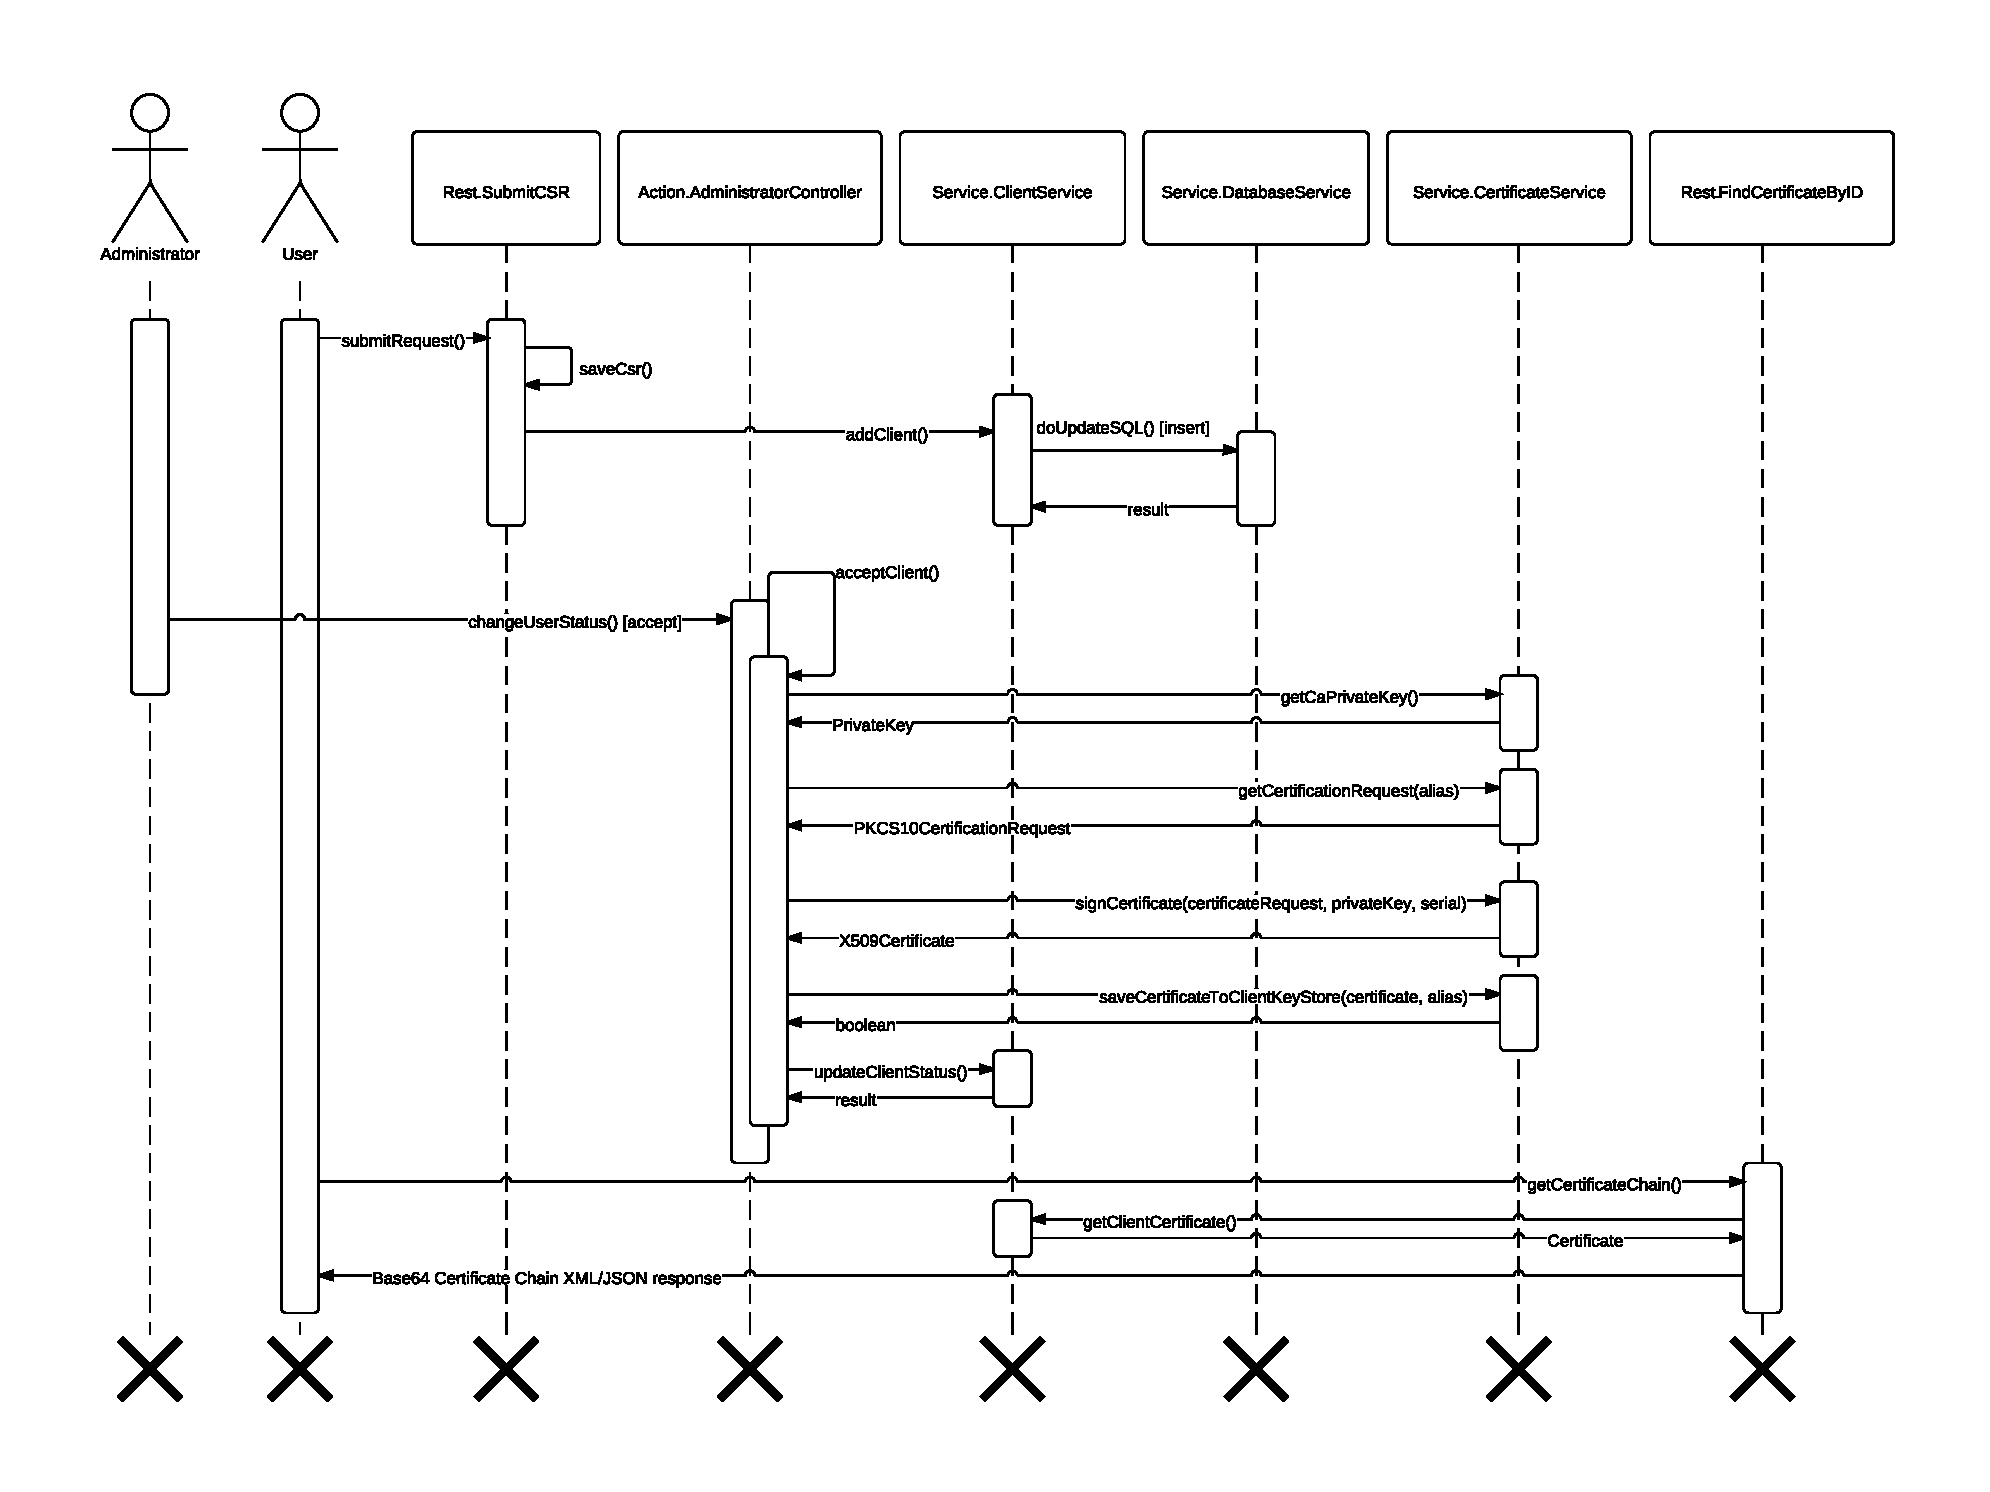
\includegraphics[height=0.80\textheight,keepaspectratio]{DomoTopSequenceDiagram_without_title.pdf}
  \label{fig:tls}
  \caption{DomoTop Sequence Diagram - Afhandelen van een request via een TLS
  capable OpenRemote Controller}
\end{figure}
\end{landscape}

\newpage
\subsection{Bijlage 3: Onderzoeksdocument PlugTop}
Het onderzoeksdocument PlugTop is bijgevoegd als bijlage aan het
afstudeerverslag.

\newpage
\subsection{Bijlage 4: Onderzoeksdocument Beveiliging OpenRemote}
Het onderzoeksdocument 'Research Security' is als bijlage toegevoegd aan dit document.

\newpage
\subsection{Bijlage 5: Onderzoeksdocument Domotica Protocollen}
Het onderzoeksdocument Domotica Protocollen is als bijlage toegevoegd aan dit
document.

\newpage
\subsection{Bijlage 6: Onderzoeksdocument OpenRemote}
Het onderzoeksdocument OpenRemote is als bijlage toegevoegd aan dit
afstudeerverslag.

\end{document}
